\documentclass{ta-its}
\usepackage{hyperref}
\usepackage{listings}
\usepackage{float}
\usepackage{wrapfig}
\usepackage{multirow}

\title{Rancang Bangun Perangkat Lunak Internet \textit{Acces Management} Berbasis Kontainer}{Design and Implementation of Internet Access Management Software Using Container}{KI141502} 

% \author{Nama Lengkap}{NRP}
\author{Fourir Akbar}{05111440000115}

% \supervisorOne{Nama Pembimbing Satu}{NIP}
% \supervisorTwo{Nama Pembimbing Dua}{NIP}
\supervisorOne{Royyana Muslim Ijtihadie, S.Kom, M.Kom, PhD}{197708242006041001}
\supervisorTwo{Bagus Jati Santoso, S.Kom., Ph.D}{051100116}

% \degree{Nama Gelar}{Bidang Studi}{Program Studi}{Jurusan}{Jurusan (English)}{Fakultas}{Fakultas Singkatan}{Fakultas (English)}
\degree{Sarjana Komputer}{Komputasi Berbasis Jaringan}{S1}{Departemen Informatika}{Informatics}{Teknologi Informasi}{FTIf}{Information Technology}

% \time{bulan}{tahun}
\time{Juni}{2018}


\begin{document}
% Ubah kode sumber romawi menjadi arabic
\renewcommand{\thelstlisting}{\arabic{chapter}.\arabic{lstlisting}}
  \frontmatter 
    \maketitle
    \legalityPaper
    \begin{abstrak}
	\indent Saat ini penggunaan kontainer docker dalam dunia teknologi sangat banyak dilakukan. Kontainer docker merupakan operating-system-level virtualization untuk menjalankan beberapa sistem linux yang terisolasi (kontainer) pada sebuah host. Kontainer berfungsi untuk mengisolasi aplikasi atau servis dan dependensinya. Untuk setiap servis atau aplikasi yang terisolasi dibutuhkan satu kontainer pada server host yang ada dan setiap kontainer akan menggunakan sumber daya yang ada pada server host selama kontainer tersebut menyala.\\
    	\indent Dalam kasus ini, setiap user yang mengakses atau menggunakan jaringan ITS merupakan satu servis yang nantinya akan dibuatkan satu kontainer pada server host. Hal ini dapat mempermudah manajemen dari masing-masing user, contohnya manajemen bandwith, hak akses, waktu, dan lain sebagainya. Jika user telah selesai mengakses atau menggunakan jaringan ITS, maka kontainer pada user tersebut akan di-destroy, sehingga hal ini dapat meringankan beban server.\\

\noindent \textbf{Kata-Kunci}:  Docker, Internet Access Management, Kontainer
\end{abstrak}

\cleardoublepage
\begin{abstract}
	\indent Nowadays, docker containers have been widely used in the word of technology. The docker containers is an operating system level virtualization to run some isolated linux systems (containers) on a host. Containers are used to isolate applications or services and its dependencies. For every service or app that isolated it takes one container on the existing host server and each container will use the existing resources on the host server as long as the container is on.
	
	In this case, any user accessing or using ITS network is one service that a container will be created on the host server. This can simplify management of each user, for example bandwidth management, access rights, time, and many more. If the user has finished accessing or using the the network ITS, then the container on the user will be destroyed, so this can reduce the server load. \\

\noindent \textbf{Keywords}:  \textit{Container, Docker, Internet Access Management}.
\end{abstract}
    \chapter{KATA PENGANTAR}
	Puji syukur Penulis panjatkan kepada Allah SWT. atas pimpinan, penyertaan, dan karunia-Nya sehingga Penulis dapat menyelesaikan Tugas Akhir yang berjudul \textbf{Rancang Bangun Perangkat Lunak Internet \textit{Acces Management} Berbasis Kontainer}. Pengerjaan Tugas Akhir ini merupakan suatu kesempatan yang sangat baik bagi penulis. Dengan pengerjaan Tugas Akhir ini, penulis bisa belajar lebih banyak untuk memperdalam dan meningkatkan apa yang telah didapatkan penulis selama menempuh perkuliahan di Teknik Informatika ITS. Dengan Tugas Akhir ini penulis juga dapat menghasilkan suatu implementasi dari apa yang telah penulis pelajari.
        Selesainya Tugas Akhir ini tidak lepas dari bantuan dan dukungan beberapa pihak. Sehingga pada kesempatan ini penulis mengucapkan syukur dan terima kasih kepada:
  \begin{enumerate}
    \item Bapak, Mama, dan keluarga Penulis yang selalu memberikan perhatian, dorongan dan kasih sayang yang menjadi semangat utama bagi diri Penulis sendiri baik selama penulis menempuh masa perkuliahan maupun pengerjaan Tugas Akhir ini.
    \item Bapak Royyana Muslim Ijtihadie, S.Kom., M.Kom., PhD. selaku Dosen Pembimbing yang telah banyak meluangkan waktu untuk memberikan ilmu, nasihat, motivasi, pandangan dan bimbingan kepada Penulis baik selama Penulis menempuh masa kuliah maupun selama pengerjaan Tugas Akhir ini.
    \item Bagus Jati Santoso, S.Kom., PhD. selaku dosen pembimbing yang telah memberikan ilmu, dan masukan kepada Penulis.
    \item Seluruh tenaga pengajar dan karyawan Jurusan Teknik Informatika ITS yang telah memberikan ilmu dan waktunya demi berlangsungnya kegiatan belajar mengajar di Jurusan Teknik Informatika ITS.
    \item Seluruh teman Penulis di Jurusan Teknik Informatika ITS yang telah memberikan dukungan dan semangat kepada Penulis selama Penulis menyelesaikan Tugas Akhir ini.
    \item Teman-teman, Kakak-kakak dan Adik-adik \textit{administrator} Laboratorium Arsitektur dan Jaringan Komputer yang selalu menjadi teman untuk berbagi ilmu.
  \end{enumerate}

  Penulis menyadari bahwa Tugas Akhir ini masih memiliki banyak kekurangan. Sehingga dengan kerendahan hati, penulis mengharapkan kritik dan saran dari pembaca untuk perbaikan ke depannya.


  \hfill Surabaya, Juni 2018 \\ \\ 


  \hfill Fourir Akbar

\cleardoublepage % Mengisi penanda halaman genap yang kosong


    \tableofcontents % Daftar isi
    \listoftables % Daftar tabel
    \listoffigures % Daftar gambar
    \lstlistoflistings % Daftar source code 

  \mainmatter % Halaman utama, dengan judul BAB X
    \chapter{PENDAHULUAN}
  Pada bab ini akan dipaparkan mengenai garis besar Tugas Akhir yang meliputi latar belakang, tujuan, rumusan dan batasan permasalahan, metodologi pembuatan Tugas Akhir, dan sistematika penulisan.
  
  \section{Latar Belakang}
    Saat ini penggunaan kontainer \textit{docker} dalam dunia tekonologi sangat banyak dilakukan. Kontainer \textit{docker} merupakan \textit{operating-system-level virtualization} untuk menjalankan beberapa sistem linux yang terisolasi (kontainer) pada sebuah \textit{host} atau \textit{server}. Kontainer berfungsi untuk mengisolasi aplikasi atau servis dan dependensinya.\\
	\indent Untuk setiap servis atau aplikasi yang terisolasi, dibutuhkan satu kontainer pada \textit{server} host yang ada. Dalam kasus ini, setiap satu \textit{client} yang mengakses atau menggunakan jaringan ITS merupakan satu servis yang nantinya akan dibuatkan satu kontainer pada \textit{server host}. Hal ini dapat mempermudah manajemen dari masing-masing \textit{client}, contohnya manajemen hak akses, waktu, maupun melihat \textit{access log} dan lain sebagainya.
	
	Setiap \textit{client} yang akan menggunakan jaringan ITS, akan diarahkan ke sebuah halaman \textit{login}. Setelah \textit{client} tersebut berhasil \textit{login}, barulah \textit{client} tersebut dapat mengakses internet.

\section{Rumusan Masalah}
	Berikut beberapa hal yang menjadi rumusan masalah dalam tugas akhir ini:
	\begin{enumerate}
	 \item Bagaimana cara mengarahkan \textit{traffic} dari \textit{client} ke halaman \textit{login}?
	 \item Bagaimana cara membuat sebuah kontainer \textit{docker} secara otomatis ketika terdapat \textit{client} yang terhubung dengan jaringan ITS?
	 \item Bagaimana cara mengarahkan \textit{traffic} dari \textit{client} ke kontainer \textit{docker} yang sesuai?
	 \item Bagaimana cara mengetahui apa saja yang diakses oleh \textit{client}?
	 \item Bagaimana perbandingan performa antara IAM konvensional dengan IAM berbasi kontainer?
	\end{enumerate}

	\section{Batasan Masalah}
	 Dari permasalahan yang telah diuraikan di atas, terdapat beberapa batasan masalah pada tugas akhir ini, yaitu:
	\begin{enumerate}
     \item Satu \textit{client} yang berhasil \textit{login} akan disediakan satu kontainer \textit{docker}.
     \item Kontainer yang digunakan adalah \textit{docker}.
	 \item Parameter untuk mengetahui apa saja yang diakses oleh \textit{client} adalah \textit{access log} dari \textit{client} tersebut.
	 \item Setiap \textit{client} mendapatkan IP \textit{private}.
     \item Performa yang diukur adalah \textit{response time}.
     \item Bahaasa pemrograman yang digunakan adalah Python.
	\end{enumerate}
    
   \section{Tujuan}
	Tugas akhir dibuat dengan beberapa tujuan. Berikut beberapa tujuan dari pembuatan tugas akhir:
	\begin{enumerate}
	 \item Mengetahui cara untuk mengarahkan \textit{traffic} dari \textit{client} ke halaman \textit{login}.
	 \item Mengimplementasikan metode untuk membuat sebuah kontainer terhadap \textit{client} yang telah berhasil \textit{login} ke jaringan ITS.
	 \item Mengetahui cara untuk mengarahkan \textit{traffic} dari \textit{client} ke kontainer \textit{docker} yang sesuai.
	 \item Mengetahui apa saja yang diakses oleh \textit{client}.
	 \item Mengetahui perbandingan performa antara IAM konvensional dengan IAM berbasis kontainer.
	\end{enumerate}
     
     \section{Manfaat}
	 Tugas akhir dibuat dengan beberapa manfaat. Berikut beberapa manfaat dari pembuatan tugas akhir:
	 \begin{enumerate}
	  \item Mengetahui cara untuk mengarahkan \textit{traffic} dari \textit{client} ke halaman \textit{login}.
	  \item Mengethaui cara untuk mengarahkan \textit{traffic} dari \textit{client} ke kontainer \textit{docker} yang sesuai.
	  \item Mempermudah pengecekan \textit{access log} dari setiap \textit{client}.
	  \item Mengetahui apa saja yang diakses oleh \textit{client} yang menggunakan jaringan ITS.
	  \item Meringankan beban dari penggunaan \textit{server} di ITS karena penggunaan kontainer \textit{docker} lebih ringan.
	 \end{enumerate}      
     
     \section{Metodologi}
     Metodologi yang digunakan pada pengerjaan Tugas Akhir ini
adalah sebagai berikut:
     \subsection{Studi literatur}
     Studi literatur merupakan langkah yang dilakukan untuk mendukung dan memastikan setiap tahap pengerjaan tugas akhir sesuai dengan standar dan konsep yang berlaku. Pada tahap studi literatur ini, akan dilakukan studi mendalam mengenai kontainer \textit{docker}, \textit{flask}, \textit{mitmproxy}, dan pembuatan aturan dengan menggunakan \textit{iptables}. Adapun literatur yang dijadikan sumber berasal dari paper, buku, materi perkuliahan, forum serta artikel dari internet.

\subsection{Desain dan Perancangan Sistem}
Tahap ini meliputi perancangan sistem berdasarkan studi literatur dan pembelajaran konsep. Tahap ini merupakan tahap yang paling penting dimana bentuk awal aplikasi yang akan diimplementasikan didefinisikan. Pada tahapan ini dibuat kasus penggunaan yang ada pada sistem, arsitektur sistem, serta perencanaan implementasi pada sistem.
\subsection{Implementasi Sistem}
Implementasi merupakan tahap membangun implementasi rancangan sistem yang telah dibuat. Pada tahapan ini merealisasikan apa yang telah didesain dan dirancang pada tahapan sebelumnya, sehingga menjadi sebuah sistem yang sesuai dengan apa yang telah direncanakan.
\subsection{Uji Coba dan Evaluasi}
Pada tahapan ini dilakukan uji coba terhadap sistem yang telah dibuat. Pengujian dan evaluasi akan dilakukan dengan melihat kesesuaian dengan perencanaan. Selain itu, tahap ini juga akan melakukan uji performa sistem dan melakukan perbandingan dengan metode lain untuk mengetahui efisiensi penggunaan sumber daya serta evaluasi berdasarkan hasil uji performa tersebut. 

\section{Sistematika Laporan}
Buku tugas akhir ini bertujuan untuk mendapatkan gambaran dari pengerjaan tugas akhir ini. Selain itu, diharapkan dapat berguna bagi pembaca yang berminat melakukan pengambangan lebih lanjut. Secara garis besar, buku tugas akhir ini terdiri atas beberapa bagian seperti berikut:
\begin{enumerate}

\item \textbf{Bab I} \indent \textbf{Pendahuluan} \\        
\indent \indent Bab yang berisi latar belakang, tujuan, manfaat, permasalahan, batasan masalah, metodologi yang digunakan dan sistematika laporan.
\\
\item \textbf{Bab II} \indent \textbf{Dasar Teori}
\\
\indent \indent Bab ini berisi penjelasan secara detail mengenai dasar-dasar penunjang dan teori-teori yang yang digunakan dalam pembuatan tugas akhir ini.
\\
\item \textbf{Bab III} \indent \textbf{Desain dan Perancangan}
\\
\indent \indent Bab ini berisi tentang analisis dan perancangan sistem yang dibuat, termasuk di dalamnya mengenai analisis kasus penggunaan, desain arsitektur sistem, dan perancangan implementasi sistem.
\\
\item \textbf{Bab IV} \indent \textbf{Implementasi}
\\
\indent \indent Bab ini membahas implementasi dari desain yang telah dibuat pada bab sebelumnya. Penjelasan berupa pemasangan alat dan kode program yang digunakan untuk mengimplementasikan sistem.
\\
\item \textbf{Bab V} \indent \textbf{Uji Coba dan Evaluasi}
\\
\indent \indent Bab ini membahas tahap-tahap uji coba serta melakukan evaluasi terhadap sistem yang dibuat.
\\
\item \textbf{Bab VI} \indent \textbf{Kesimpulan dan Saran}
\\
\indent \indent Bab ini merupakan bab terakhir yang memberikan kesimpulan dari hasil percobaan dan evaluasi yang telah dilakukan. Pada bab ini juga terdapat saran bagi pembaca yang berminat untuk melakukan pengembangan lebih lanjut.    
\end{enumerate}
    \chapter{LANDASAN TEORI}

 \section{Python}
	 Python adalah bahasa pemrograman interpretatif multiguna dengan prinsip agar sumber kode yang dihasilkan memiliki tingkat keterbacaan yang baik. Python diklaim sebagai bahasa yang menggabungkan kapabilitas, kemampuan, dengan sintaksis kode yang sangat jelas, dan dilengkapi dengan fungsionalitas pustaka standar yang besar serta komprehensif. Python mendukung beragam paradigma pemrograman, seperti pemrograman berorientasi objek, pemrograman imperatif, dan pemrograman fungsional. Python dapat digunakan untuk berbagai keperluan pengembangan perangkat lunak dan dapat berjalan di berbagai platform sistem operasi \cite{bab2-python} \\

 \section{Flask}
	 Flask adalah sebuah kerangka kerja web. Artinya, Flask menyediakan perangkat, pustaka, dan teknologi yang memungkinkan seorang pengembang untuk membangun aplikasi berbasis web. Aplikasi web yang bisa dibangun bisa berupa sebuah halaman web, blog, wiki, bahkan untuk web komersial. Flask dibangun berbasiskan pada Werkzeug, Jinja 2, dan MarkupSafe yang mana menggunakan bahasa pemrograman Python sebagai basisnya. Flask sendiri pertama kali dikembangkan pada tahun 2010 dan didistribusikan dengan lisensi BSD \\
	 \indent Flask termasuk sebagai perangkat kerja mikro karena tidak membutuhkan banyak perangkat atau pustaka tertentu agar bisa bekerja. Flask tidak menyediakan fungsi untuk melakukan interaksi dengan basis data, tidak mempunya validasi \textit{form} atau fungsi lain yang umumnya bisa digunakan dan disediakan pada sebuah kerangka kerja web. Meskipun memiliki kemampuan yang minim, tapi Flask mendukung dan memberikan kemudahan bagi pengembang untuk menambahkan pustaka sendiri untuk mendukung aplikasinya. Berbagai pustaka seperti validasi \textit{form}, mengunggah file, berbagai macam teknologi autentifikasi bisa digunakan dan tersedia untuk Flask. Bahkan pustaka-pustaka pendukung tersebut lebih sering diperbarui dibandingkan dengan Flasknya sendiri.
	 
 \section{\textit{Gunicorn}}
 \textit{Gunicorn} atau '\textit{Green Unicorn}' adalah \textit{Python} WSGI HTTP \textit{Server} untuk UNIX. Fungsi dari \textit{Gunicorn} ini adalah sebagai pelayan sebuah aplikasi atau sebagai server dari sebuah perangkat lunak yang dikembangkan oleh pengembang.
 
 \textit{Gunicorn} sendiri merupakan salah satu dari sekian banyak \textit{WSGI Server}. Keunggulan dari \textit{Gunicorn} sendiri adalah, \textit{Gunicorn} mampu menangani atau kompatibel dengan berbagai macam kerangka kerja web, sangat mudah untuk diimplementasikan, hanya membutuhkan sedikit sumber daya dari \textit{server} yang terpasang \textit{Gunicorn}, dan juga kerja dari \textit{Gunicorn} yang sangat cepat.
 
 \textit{Gunicorn} mengimplementasikan spesifikasi standar \textit{server WSGI PEP3333} sehingga dapat menjalankan perangkat lunak berbasis \textit{web} yang dikembangkan dengan bahasa pemrograman \textit{python}. Sebagai contoh, perangkat lunak berbasis web yang digunakan oleh penulis menggunakan kerangka kerja \textit{flask}, maka \textit{Gunicorn} dapat menanganinya.
 
 \section{\textit{Supervisor}}
 \textit{Supervisor} adalah sistem yang berbasis \textit{client} atau server, yang memungkinkan penggunanya utuk memantau dan juga mengontrol sejumlah proses pada sistem operasi untuk UNIX. Beberapa faktor terbentuknya \textit{supervisor} antara lain adalah, kenyamanan, ketepatan, delegasi, dan proses grup dalam menggunakan perangkat lunak \textit{supervisor}. Beberapa keunggulan dari perangkat lunak \textit{supervisor} antara lain, konfigurasi yang sederhana, proses yang terpusat, efisien, dapat diperluas penggunaannya, dan juga kompatibel dengan berbagai macam sistem operasi. Komponen dari \textit{supervisor} terbagi menjadi dua, antara lain sebagai berikut.
 
 \subsection{\textit{Supervisord}}
 \textit{Supervisord} merupakan bagian dari \textit{supervisor} yang bertanggung jawab untuk memulai \textit{child programs} atas permintaannya sendiri, menanggapi perintah dari \textit{client}, melakukan \textit{restart} secara otomatis ketika terjadi kerusakan pada proses, mencatat bagian dari proses \texttt{stdout} dan \texttt{stderr} \textit{output}, juga menghasilan dan menangani \textit{events} yang berhubungan dengan bagian-bagian yang digunakan selama \textit{subprocess} tersebut berjalan.
 
 \subsection{\textit{Supervisorctl}}
 \textit{Supervisorctl} merupakan bagian dari \textit{command-line} yang digunakan oleh \textit{client}. \textit{Supervisorctl} menyediakan antarmuka yang mirip dengan fitur \textit{shell} yang disediakan oleh \textit{supervisord}. Dari \textit{supervisorctl}, pengguna dapat terhubung dengan proses \textit{supervisord} yang berbeda satu per satu, mendapatkan status dari \textit{subprocess} yang telah dikontrol, menghentikan atau memulai \textit{subprocess} yang telah dikontrol, dan juga mendapatkan semua daftar proses yang berjalan pada \textit{supervisord}.
 
 \textit{Command-line} dari \textit{client} berhubungan ke \textit{server} melalui \textit{socket domain} UNIX atau melalui \textit{socker internet} (TCP). \textit{Server} dapat menyatakan bahwa \textit{client} harus memberikan \textit{autentifikasi} sebelum mengizinkannya untuk melakukan sebuah perintah. Proses \textit{client} biasanya menggunakan \textit{file} konfigurasi yang sama dengan \textit{server}. 
 
 \section{\textit{Nginx}}
 Nginx adalah sebuah perangkat lunak yang bisa digunakan untuk \textit{web server}, \textit{load balancer}, dan \textit{reverse proxy}. Nginx terkenal karena stabil, memiliki tingkat performa tinggi dan konsumsi sumber daya yang minim. Pada kasus saat terjadi koneksi dalam jumlah yang banyak secara bersamaan, penggunaan \textit{memory}, CPU, dan sumber daya sistem yang lain sangat kecil dan stabil. \cite{chi_web_2012}\\
 \indent Nginx bisa digunakan untuk menyajikan kontent HTTP yang dinamis menggunakan FastCGI, SCGI untuk menangani scripts, aplikasi WSGI , dan bisa juga digunakan sebagai sebuah \textit{load balancer}. Nginx menggunakan \textit{asynchronous event-driven} untuk menangani permintaan. Dengan menggunakan model ini bisa, pengembang bisa melakukan predeksi kinerja Nginx saat terjadi jumlah permintaan yang banyak.
	 
 \section{\textit{Iptables}} 
 \textit{Firewall} merupakan sebuah mekanisme wajib \textit{access} kontrol antar jaringan ataupun antar sistem. \textit{Firewall} ini sangat penting karena bertujuan untuk memastikan keamanan dari sebuah jaringan. \textit{Firewall} dapat menjadi \textit{filter} yang sangat sederhana dan mudah digunakan, tetapi \textit{firewall} juga dapat menjadi \textit{filter} yang sangat penting bagi sebuah jalan keluar suatu jaringan. Prinsip dari penggunaan \textit{firewall} tetaplah sama, dimana penggunaannya untuk \textit{monitoring} dan \textit{filtering} semua pertukaran informasi di jaringan \textit{internal} dan juga di jaringan \textit{external}.
 
 \textit{Netfilter} / \textit{iptables} merupakan sebuah sistem \textit{firewall} berbasis linux yang mempunyai fungsi yang sangat berguna. \textit{Netfilter} / \textit{iptables kernel} menggunakan sebuah mekanisme baru, bernama \textit{iptables}. \textit{Ipbtales} sendiri merupakan sebuah perangkat lunak atau alat yang dapat melakukan manajemen \textit{filter} dari sebuah paket yang ada pada suatu \textit{kernel}. \textit{Iptables} mempunyai \textit{table} dan juga \textit{chain} dari masing-masing \textit{table}. \textit{Table} pada \textit{iptables} terdiri dari tiga, atau juga bisa disebut \textit{iptables} memiliki tiga fungsi utama, antara lain menjadi penyaring paket, mentranslasikan suatu alamat, dan melakuakn penghalusan paket seperti TTL, TOS, dan MARK.
 
 \textit{Filter table} merupakan sebuah konfigurasi \textit{default} dari \textit{iptables}, dimana pada \textit{filter table} terdapat tiga \textit{chain}, antara lain \textit{chain} INPUT, FORWARD, dan OUTPUT. \textit{NAT table} berfungsi untuk merubah tujuan dari sumber dari sebuah paket. Pada \textit{NAT table} terdapat dua \textit{chain}, antara lain \textit{chain} PREROUTING dan POSTROUTING. \textit{Mangle table} berfungsi untuk menghaluskan paket atau juga dapat mengubah isi dari sebuah data kecuali IP \textit{address} dan \textit{port address}.Pada \textit{mangle table} terdapat dua \textit{chain}, antara lain POSTROUTING dan OUTPUT.
	 
 \section{MySQL}
	 MySQL adalah sebuah perangkat lunak terbuka untuk melakukan manajemen basis data SQL atau DBMS. MySQL ditulis dalam bahasa pemrograman C dan C++. MySQL merupakan salah satu perangkat lunak terbuka yang banyak disukai oleh pengembang dan digunakan dalam banyak aplikasi web. Parser SQL yang digunakan ditulis dalam bahasa pemrograman yacc. MySQL bekerja pada banyak \textit{platform}, seperti  FreeBSD, HP-UX, Linux, macOS, Microsoft Windows, NetBSD, OpenBSD, OpenSolaris, Oracle Solaris, dan SunOS. MySQL tersedia sebagai perangkat lunak gratis di bawah lesensi \textit{GNU General Public License} (GPL), tetapi juga tersedia lisensi komersial untuk kasus-kasus dimana penggunanya tidak cocok dengan penggunaan GPL.\\
	 \indent Setiap pengguna dapat secara bebas menggunakan MySQL, namun dengan batasan perangkat lunak tersebut tidak boleh dijadikan produk turunan yang bersifat komersial. MySQL sebenarnya merupakan turunan salah satu konsep utama dalam basis data yang telah ada sebelumnya, yaitu SQL (\textit{Structured Query Language}). SQL adalah sebuah konsep pengoperasian basis data, terutama untuk proses pemilihan atau seleksi dan pemasukan data, yang memungkinkan pengoperasian data dikerjakan dengan mudah.\\
	 \indent Kehandalan suatu sistem basis data dapat diketahui dari cara kerja pengoptimasiannya dalam melakukan proses perintah-perintah SQL yang dibuat oleh pengguna maupun program-program aplikasi yang memanfaatkannya. Sebagai \textit{server} basis data, MySQL mendukung operasi basis data transaksional maupun operasi basis data non-transaksional. Pada modus operasi non-transaksional, MySQL dapat dikatakan handal dalam hal unjuk kerja dibandingkan \textit{server} basis data kompetitor lainnya. Namun pada modus non-transaksional tidak ada jaminan atas reliabilitas terhadap data yang tersimpan, karenanya modus non-transaksional hanya cocok untuk jenis aplikasi yang tidak membutuhkan reliabilitas data seperti aplikasi blogging berbasis web (wordpress), CMS, dan sejenisnya. Untuk kebutuhan sistem yang ditujukan untuk bisnis sangat disarankan untuk menggunakan modus basis data transaksional, hanya saja sebagai konsekuensinya unjuk kerja MySQL pada modus transaksional tidak secepat unjuk kerja pada modus non-transaksional.
	
	\section{\textit{Mitmproxy}}
	
	\textit{Mitmproxy} adalah sebuah sebuah \textit{interception proxy} untuk HTTP dengan antarmuka pengguna \textit{console} yang ditulis dengan bahasa \textit{Python}. \textit{Mitmproxy} merupakan sebuah perangkat lunak yang interaktif dimana \textit{Mitmproxy} memungkinkan dapat memotong dan memodifikasi HTTP \textit{requests} atau \textit{response} dengan sangat cepat.
	
	\textit{Mitmproxy} ada sebuah \textit{proxy} berkemampuan SSL yang berfungsi sebagai \textit{man-in-the-middle} untuk komunikasi HTTP dan HTTPS. Untuk dapat mengetahui atau memodifikasi komunikasi HTTPS, \textit{mitmproxy} berupra-pura menjadi \textit{server} ke \textit{client} dan \textit{client} ke server, sementara itu \textit{mitmproxy} diposisikan di tengah-tengah berfungsi untuk menerjemahkan lalu lintas dari keduanya. \textit{Mitmproxy} menghasilkan sertifikat \textit{on-the-fly} untuk mengetahui \textit{client} agar percaya bahwa mereka berkomunikasi dengan \textit{server}.
	
	Pertama kali \textit{mitmproxy} dimulai, maka akan menghasilkan sertifikat SSL yang berada pada \texttt{~/.mitmproxy/cert.pem}. Sertifikat ini akan digunakan untuk \textit{browser-side}. Karena tidak akan cocok dengan \textit{domain} yang \textit{client} kunjungi, dan tidak akan memverifikasi terhadap otoritas sertifikasi, \textit{client} harus menambahkan pengecualian untuk setiap situs yang \textit{client} kunjungi. Permintaan SSL dicegat dengan hanya mengamsumsikan bahwa semua permintaan \texttt{CONNECT} adalah HTTPS. Sambungan dari \textit{browser} dibungkus SSL, dan kita membaca permintaan dengan berpura-pura menjadi \textit{server} yang menghubungkan.
	
	\section{\textit{VirtualBox}}
	\textit{VirtuaBox} merupakan salah satu produk perangkat lunak yang sekarang dikembangkan oleh Oracle. Aplikasi ini pertama kali dikembangkan oleh perusahaan Jerman, Innotek GmbH. Februari 2008, Innotek GmbH diakusisi oleh Sun Micorsystems. Sun Microsystems kemudian juga diakuisisi oleh Oracle. \textit{VirtualBox} berfungsi untuk melakukan virtualisasi sistem operasi. \textit{VirtualBox} juga dapat digunakan untuk membuat virtualisasi jaringan komputer sederhana. Penggunaan \textit{VirtualBox} ditargetkan untuk \textit{server}, desktop, dan penggunaan \textit{embedded}.
	
	Berdasarkan jenis VMM yang ada, \textit{VirtualBox} merpakan jenis \textit{hypervisor type 2}. \textit{VirtualBox} sendiri memiliki berbagai macam kegunaan, diantaranya \textit{VirtualBox} dapat memainkan semua sistem  operasi baik itu menggunakan windows, linux, atau turunan linux lainnya. \textit{VirtualBox} juga dapat dipergunakan untuk mengujicoba OS baru. \textit{VirtualBox} juga dapat digunakan sebgai media untuk membaut simulasi jaringan.
	
	\section{\textit{Framework} Laravel}
	
	Laravel adalah sebuah \textit{framework} PHP yang dibangun dengan konsep MVC (\textit{Model View Controller}). MVC adalah sebuah pendekatan perangkat lunak yang memisahkan aplikasi logika dari presentasi. MVC memisahkan aplikasi berdasarkan komponen-komponen aplikasi, seperti: manipulasi data, \textit{controller}, dan \textit{user interface}.
	\begin{enumerate}
	\item \textit{Model} berisi fungsi-fungsi yang membantu seseorang dalam pengelolaan data, dan lain-lain.
	\item \textit{View} adalah bagian yang mengatur tampilan ke pengguna. Bisa dikatakan berupa halaman web.
	\item \textit{Controller} merupakan bagian yang menjembatani \textit{model} dan \textit{view}.
	\end{enumerate}
	Rancang Bangun Perangkat Lunak Internet \textit{Access Management} Berbasis Kontainer
	Dalam pembangunan perangkat lunak internet \textit{access management} berbasis kontainer, Laravel digunakan sebagai \textit{framework} untuk pembangunan web sebagai halaman \textit{administrator}. Salah satu fitur yang mendukung proses pengembangan dari Laravel adalah Eloquent ORM. Misalkan, dibutuhkan untuk mengambil semua data yang ada pada tabel \texttt{Kontainer}, maka yang perlu dilakukan hanya membuat sebuah \textit{class model} bernama \textit{Kontainer}. Laravel sendiri dikembangkan secara khusus untuk PHP 7.0. Jadi \textit{framework} ini bisa memanfaatkan berbagai macam kelebihan yang dimiliki PHP versi terbaru tersebut. Tidak ada \textit{backward compatibility} dengan PHP versi sebelumnya.
	
		
	\section{\textit{Docker}}
	Docker adalah sebuah aplikasi yang bersifat \textit{open source} yang berfungsi sebagai wadah untuk memasukkan sebuah perangkat lunak secara lengkap beserta semua hal yang dibutuhkan oelh perangkat lunak tersebut agar dapat berfungsi sebagaimana mestinya. \textit{Docker} dapat dijalankan di berbagai sistem operasi, pengembang dapat dengan mudah menggunakan layanan \textit{docker} melalui \texttt{https://hub.docker.com} untuk mengunduh \textit{imaes} ataupun membuat \textit{images} yang diinginkan. Perbedaan antara \textit{docker} dan \textit{virtual machine} ditunjukkan pada gambar \ref{contohDocker}
	
	\begin{figure}[H] % h = pasti berada di bawah teks yang ada di atas
	\centering
	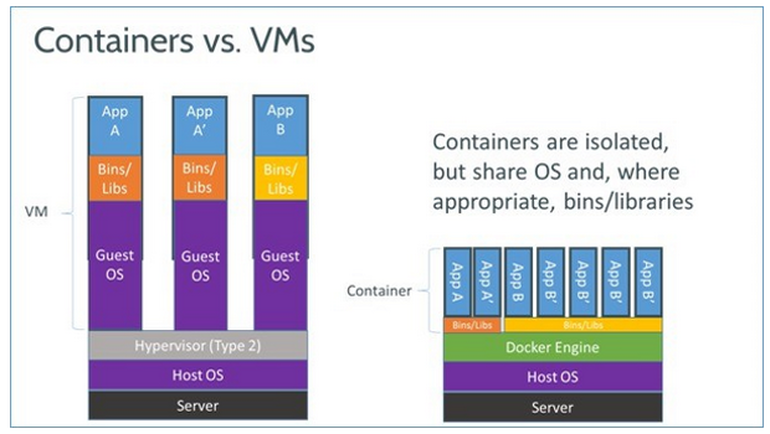
\includegraphics[width=\linewidth]{images/bab2/docker-vm-container}
	\caption{Perbandingan \textit{docker} dan virtual machine}
	\label{contohDocker}
	\end{figure}
	
	\subsection{\textit{Docker Container}}
	\textit{Docker container} atau kontainer \textit{docker} bisa dikatakan sebagai sebuah wadah atau tempat, dimana kontainer \textit{docker} ini dibuat dengan menggunakan \textit{docker image}. Saat kontainer \textit{docker} dijalankan, maka akan terbentu sebuah \textit{layer} di atas \textit{docker image}.Contohnya saat menggunakan \textit{image} Ubuntu, kemudian membuat sebuah kontainer \textit{docker} dari \textit{image} Ubuntu tersebut dengan nama mitmproxy-ubuntu. Setelah itu dilakukan pemasangan sebuah perangkat lunak, misalnya \textit{mitmproxy}, maka secara otomatis kontainer \textit{docker} mitmproxy-ubuntu akan berada di atas \textit{layer image} Ubuntu, dan diatasnya lagi merupakan \textit{layer mitmproxy} berada. \textit{Docker Kontainer} atau Kontainer \textit{docker} ke depannya dapat digunakan untuk menghasilkan sebuah \textit{docker images}. \textit{Docker images} yang dihasilkan dari kontainer \textit{docker} itu sendiri nantinya dapat digunakan kembali untuk membuat kontainer \textit{docker} yang lainnya.
	
	\subsection{\textit{Docker Images}}
	\textit{Docker images} adalah sebuah \textit{blueprint} atau rancangan dasar dari sebuah perangkat lunak berbasis \textit{docker} yang bersifat \textit{read-only}. \textit{Blueprint} ini sendiri merpakan sebuah sistem operasi atau sistem operasi yang telah dipasang berbagai perangkat lunak dan pustaka pendukung. \textit{Docker iamges} berfungsi untuk membuat kontainer \textit{docker}, dimana dengan menggunakan satu \textit{docker iamge} dapat dibuat lebih dari satu kontainer \textit{docker}. \textit{Docker image} sendiri dapat menyelesaikan permasalahan yang dikenal dengan "\textit{dependency hell}", dimana sulitnya untuk melengkapi dependensi sebuah perangkat lunak. Permasalahan tersebut dapat diselesaikan karena semua kebutuhan perangkat lunak sudah berada di dalamnya.
	
	\subsection{\textit{Docker Registry}}
	\textit{Docker Registry} adalah kumpulan dari berbagai macam \textit{docker image} yang bersifat tertutup maupun terbuka yang dapat diakses di \texttt{https://hub.docker.com/} atau dapat diakses pada \textit{server} sendiri. Dengan menggunakan \textit{docker registry}, seseorang dapat menggunakan \textit{docker image} yang telah dibuat oleh orang lainnya. Hal seperti ini dapat mempermudah seseorang untuk melakukan pengembangan dan jugatransfer aplikasi.
	
    \chapter{DESAIN DAN PERANCANGAN}
  Pada bab ini dibahas mengenai analisis dan perancangan dari sistem. 
  \section{Deskripsi Umum Sistem}    
    Sistem yang akan dibuat adalah sebuah sebuah sistem yang dapat membuat sebuah kontainer \textit{docker} secara otomatis untuk setiap satu \textit{client} yang telah \textit{login} ke dalam sistem. Saat \textit{client} belum \textit{login} ke dalam sistem, maka \textit{client} tersebut akan diarahkan ke halaman \textit{login} dari sistem. Saat \textit{client} mencoba untuk \textit{login} ke dalam sistem, maka sistem akan melakukan pengecekan di dalam basis data apakah \textit{username} dan \textit{password} yang di\textit{input}kan sudah benar atau salah. 
    
    Setelah \textit{client} berhasil \textit{login} ke dalam sistem, sistem akan mengirimkan perintah untuk membuat kontainer \textit{docker} yang berisikan \textit{mitmproxy} ke \textit{docker host}. Setelah berhasil membuat kontainer \textit{docker} untuk client tersebut, maka \textit{traffic} internet dari \textit{client} tersebut akan diarahkan ke kontainer \textit{docker} berisikan \textit{mitmproxy} yang baru saja dibuat. Setelah itu akan client baru dapat untuk mengakses internet.
  
  \section{Kasus Penggunaan}
  Terdapat empat aktor dalam sistem yang akan dibuat yaitu \textit{Client}, \textit{Server Login}, \textit{Administrator}, dan \textit{Docker Host}. \textit{Client} adalah aktor yang melakukan proses \textit{login} ke dalam sistem, \textit{server login} adalah aktor yang melakukan proses permintaan penyediaan kontainer \textit{docker}, \textit{administrator} adalah aktor yang melakukan monitoring kontainer \textit{docker} yang sedang berjalan, sedangkan \textit{docker host} adalah aktor yang akan menjadi tempat penyedia kontainer dan menerima perintah penyediaan kontainer. Diagram kasus penggunaan menggambarkan kebutuhan - kebutuhan yang harus dipenuhi sistem. Diagram kasus penggunaan digambarkan pada Gambar \ref{gambarDiagramKasusPenggunaan}.
  \begin{figure}[!h] % h = pasti berada di bawah teks yang ada di atas
  \centering
  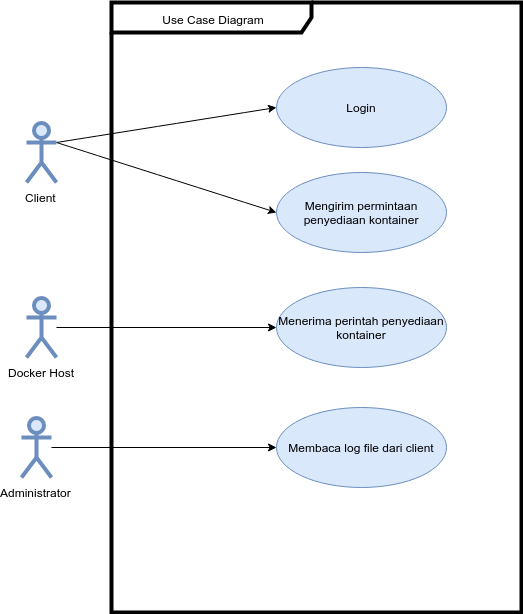
\includegraphics[width=\linewidth]{images/bab3/usecase}
  \caption{Digram Kasus Penggunaan}
  \label{gambarDiagramKasusPenggunaan}
  \end{figure}
  \\
		    		    
	Digram kasus penggunaan pada Gambar \ref{gambarDiagramKasusPenggunaan} dideskripsikan masing-masing pada Tabel \ref{tabelKodeKasusPenggunaan}.
    \begin{longtable}{|p{0.25\textwidth}|p{0.24\textwidth}|p{0.35\textwidth}|} % L = Rata kiri untuk setiap kolom, | = garis batas vertikal.

% Kepala tabel, berulang di setiap halaman
\caption{Daftar Kode Kasus Penggunaan} \label{tabelKodeKasusPenggunaan} \\
\hline
\textbf{Kode Kasus Penggunaan} & \textbf{Nama Kasus Penggunaan} & \textbf{Keterangan} \\ \hline

\endhead
\endfoot
\endlastfoot

% Isi Tabel
UC-0001 & \textit{Login} & \textit{Client} dapat \textit{login} ke dalam sistem. \\ \hline
UC-0002 & Mengirim Permintaan Penyediaan Kontainer \textit{Docker} & \textit{Server login} dapat mengirimkan permintaan penyediaan kontainer \textit{docker} pada \textit{docker host}. \\ \hline
UC-0003 & Menerima Perintah Penyediaan Kontainer \textit{Docker}  &  Proses dimana \textit{docker host} akan menerima perintah dari sistem, untuk menyediakan kontainer secara otomatis.\\ \hline
UC-0004 & Membuat Aturan untuk Mengarahkan \textit{Traffic Client}  &  Proses dimana \textit{docker host} akan membuat aturan untuk mengarahkan \textit{traffic client} ke halaman \textit{login} dari sistem atau untuk membuat aturan untuk mengarahkan \textit{traffic client} ke kontainer \textit{docker} dari tiap-tiap \textit{client}. \\ \hline
UC-0005 & Membaca \textit{Log File} dari \textit{Client}  &  Proses dimana \textit{administrator} dari sebuah jaringan dapat membaca \textit{log file} dari client secara \textit{live} ataupun juga ketika \textit{client} telah selesai menggunakannya.\\ \hline
\end{longtable}

  \section{Arsitektur Sistem}
  	Pada Sub-bab ini, dibahas mengenai tahap analisis arsitektur, analisis teknologi dan desain sistem yang akan dibangun.
    \subsection{Desain Umum Sistem}
      \indent Berdasarkan deskripsi umum sistem yang telah ditulis diatas, dapat diperoleh kebutuhan sistem ini, diantaranya :
        \begin{enumerate}
        \item Pemeriksaan data kontainer yang sudah dibuat pada \textit{docker host}.
        \item Pembuatan aturan untuk mengarahkan \textit{traffic client} ke halaman \textit{login} dari sistem.
        \item Pembuatan aturan untuk mengarhakn \textit{traffic client} ke kontainer \textit{docker} dari tiap-tiap \textit{client}.
        \item Pemasangan kontainer pada \textit{docker host}.
        \item Pembacaan \textit{log file} dari \textit{client}.
        \end{enumerate} 
      
      \indent Untuk memenuhi kebutuhan sistem tersebut, penulis membagi sistem menjadi beberapa komponen. Komponen yang akan dibangun antara lain: 
      \begin{enumerate} 
	  \item Pemeriksaan data kontainer yang sudah dibuat pada \textit{docker host}.\\
		  Berfungsi agar sistem mengetahui apakah \textit{client} dengan IP tersebut diperbolehkan mengakses internet atau tidak.
	  \item Pembuatan aturan untuk mengarahkan \textit{traffic client} ke halaman \textit{login} dari sistem.\\
		  Berfungsi untuk mengarahkan tiap \textit{client} yang belum \textit{login} ke dalam sistem ke halaman \textit{login} dari sistem. Hal ini dilakukan dengan menjalankan sebuah \textit{script} dengan menggunakan \textit{iptables} pada \textit{docker host}.
	  \item Pembuatan aturan untuk mengarahkan \textit{traffic client} ke kontainer \textit{docker} dari tiap-tiap \textit{client}.\\
		  Berfungsi untuk mengarahkan tiap \textit{client} yang telah berhasil \textit{login} ke kontainer \textit{docker} dari tiap-tiap \textit{client}. Hal ini dilakukan dengan menjalankan sebuah \textit{script} dengan menggunakan \textit{iptables} pada \textit{docker host}.
	  \item Pemasangan kontainer pada \textit{docker host}.\\
		  Berfungsi untuk memasangkan kontainer \textit{docker} pada \textit{docker host} secara otomatis. Hal ini dilakukan dengan menjalankan sebuah perintah penyediaan kontainer pada \textit{docker host}.
	  \item Pembacaan \textit{log file} dari \textit{client}.
		  Berfungsi untuk melihat apa saja yang telak diakses oleh \textit{client}. \textit{Log} yang tersimpan terdapat \textit{log} HTTP maupun \textit{log} HTTPS. Hal ini dilakukan dengan menjalankan sebuah perintah untuk melihat \textit{log file} dari suatu \textit{client}.
        
      \end{enumerate}
      
      \begin{figure}[H]
        \centering
        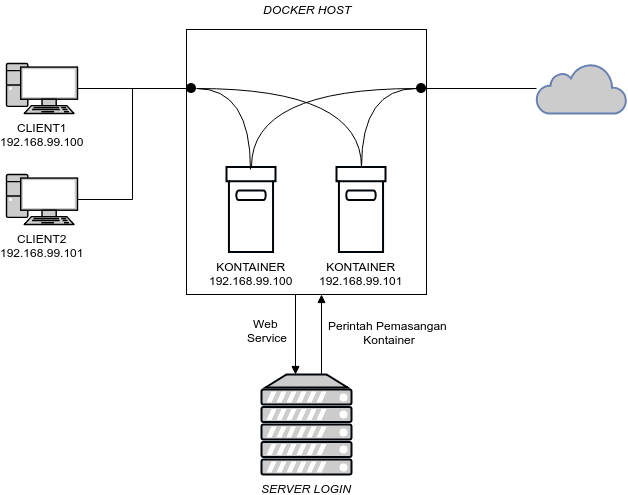
\includegraphics[width=\linewidth]{images/bab3/DIAGRAM1}
        \caption{Arsitektur Komponen Sistem}
        \label{Arsitektur Komponen Sistem}
      \end{figure}
      
    \indent Pada pada Gambar \ref{Arsitektur Komponen Sistem} ditunjukkan arsitektur sistem secara umum dengan detail-detail dari kompenen yang terdapat didalamnya. Setiap komponen tersebut akan diimplementasikan dengan teknologi pendukung yang dibutuhkan.
    
    Nantinya tiap \textit{client}  akan mempunyai satu kontainer \textit{docker} dan satu \textit{port} secara pribadi. \textit{Traffic} dari \textit{client} tersebut akan diarahkan menuju ke kontainer \textit{docker}nya dari tiap-tiap \textit{client}, setelah itu \textit{client} baru dapat mengakses itnernet.
    
    \subsection{Perancangan Pemeriksaan Data Kontainer yang Sudah Dibuat pada \textit{docker host}.}
    Pemeriksaan data kontainer yang sudah dibuat pada \textit{docker host} adalah komponen yang bertugas untuk melakukan pemeriksaan pada setiap kontainer \textit{docker} pada \textit{docker host} yang sudah dibuat. Jika pada saat dilakukan pemeriksaan ternyata belum dibuatkan kontainer \textit{docker} pada \textit{docker host}, maka \textit{client} akan diarahkan menuju ke halaman \textit{login} sistem. Setelah \textit{client} tersebut berhasil login, maka sistem akan membuat secara otomatis kontainer \textit{docker} pada \textit{docker host}. Jika pada saat dilakukan pemeriksaan ternyata sudah dibuatkan kontainer \textit{docker} pada \textit{docker host}, maka \textit{client} tersebut akan dibuatkan sebuah \textit{rules} menggunakan iptables yang berfungsi untuk mengijinkan \textit{client} tersebut mengakses internet.
    
    Dikarenakan ada beberapa kebutuhan yang harus dipenuhi, komponen pada pemeriksaan data kontainer \textit{docker} yang sudah dibuat pada \textit{docker host} dibagi lagi menadji 2 sub komponen, yaitu:
   	\begin{enumerate}
   		\item Basis Data \\
   		Basis data berfungsi sebagai tempat penyimpanan data \textit{username} dan \textit{password} yang digunakan untuk \textit{login} ke dalam sistem. Basis data juga berfungsi sebagai tempat penyimpanan data kontainer \textit{docker} yang sudah dibuat.
   		\item \textit{Web Service} \\
   		\textit{Web service} berfungsi sebagai antarmuka untuk \textit{client} ketika \textit{client} akan \textit{login} ke dalam sistem. Selain itu \textit{web service} juga berfungsi sebagai penerima permintaan dari \textit{client}, yang nantinya akan membuat sebuah kontainer \textit{docker} secara otomatis pada \textit{docker host}.
   	\end{enumerate}
   	
   	Pada tugas akhir ini, bahasa Python dipilih sebagai bahasa pemrograman yang digunakan untuk mengimplementasikannya. Lalu, pada bagian penyimpanan data atau basis data, MySQL dipilih sebagai RDBMS untuk tugas akhir ini.
   	\subsubsection{Desain Basis Data}
   	Komponen basis data berfungsi sebagai tempat penyimpanan data \textit{username} dan \textit{password} yang digunakan untuk \textit{login} ke dalam sistem. Dalam basis data ini terdapat satu entitas dan dua atribut, ditunjukkan pada Tabel \ref{tabelnrpmahasiswa}
   	\begin{longtable}{|p{0.03\textwidth}|p{0.20\textwidth}|p{0.20\textwidth}|p{0.41\textwidth}|}
   		\caption{Atribut basis data nrp-mahasiswa} \label{tabelnrpmahasiswa} \\
   		\hline
   		\textbf{No} & \textbf{Kolom} & \textbf{Tipe} & \textbf{Keterangan} \\ \hline
   		\endhead
   		\endfoot
   		\endlastfoot
   		1 & id & int(11) & Sebagai primary key pada tabel, nilai awal adalah \texttt{AUTO\_INCREMENT}. \\ \hline
   		2 & username & varchar(50) & Menunjukkan NRP dari mahasiswa yang telah terdaftar. \\ \hline
   		3 & password & varchar(50) & Menunjukkan password dari NRP mahasiswa yang telah terdaftar. \\ \hline
   		4 & isLogin & int(11) & Status apakah nrp tersebut sedang digunakan (1), atau sedang tidak digunakan (0). \\ \hline
   	\end{longtable}
   	
   	Selain itu, komponen basis data juga berfungsi sebagai tempat penyimpanan data kontainer \textit{docker} yang sudah dibuat. Dalam basis data ini terdapat satu entitas dan tiga atribut, ditunjukan pada Tabel \ref{tabelkontainer}
   	\begin{longtable}{|p{0.03\textwidth}|p{0.20\textwidth}|p{0.20\textwidth}|p{0.41\textwidth}|}
   		\caption{Atribut basis data nrp-mahasiswa} \label{tabelkontainer} \\
   		\hline
   		\textbf{No} & \textbf{Kolom} & \textbf{Tipe} & \textbf{Keterangan} \\ \hline
   		\endhead
   		\endfoot
   		\endlastfoot
   		1 & id & int(11) & Sebagai primary key pada tabel, nilai awal adalah \texttt{AUTO\_INCREMENT}. \\ \hline
   		2 & username & varchar(50) & Menunjukkan NRP dari mahasiswa yang telah berhasil dibuatkan satu kontainer \textit{docker}. \\ \hline
   		3 & ip & varchar(50) & Menunjukkan IP dari \textit{client} yang telah berhasil satu kontainer \textit{docker}. \\ \hline
   		4 & createdAt & datetime & Menunjukkan waktu pertama kali kontainer \textit{docker} tersebut dibuat. \\ \hline
   		
   	\end{longtable}
	   
   	\subsubsection{Desain \textit{Web Service}}
	Komponen \textit{web service} berfungsi untuk menyediakan antarmuka halaman \textit{login} untuk \textit{client} dan untuk mengirimkan permintaan pembuatan kontainer \textit{docker} secara otomatis pada \textit{docker host} setelah terdapat \textit{client} yang berhasil \textit{login} ke dalam sistem. Halaman \textit{login} akan menggunakan Material UI untuk mendapatkan tampilan yang sederhana dan nyaman untuk digunakan.
	
	\subsection{Perancangan Pembuatan Aturan untuk Mengarahkan \textit{Traffic Client} ke Halaman \textit{Login} dari Sistem}
	Pembuatan aturan untuk mengarahkan \textit{traffic client} ke halaman \textit{login} dari sistem adalah komponen yang bertugas untuk membelokkan \textit{traffic} dari \textit{client} yang akan menuju ke internet. Awalnya semua \textit{traffic} dari satu \textit{subnet client} tersebut akan diarahkan ke halaman \textit{login} dari sistem dengan membuat sebuah aturan menggunakan \textit{iptables}, karena asumsinya adalah belum ada \textit{client} yang berhasil \textit{login} ke dalam sistem.
   	
    \subsection{Perancangan Pemasangan Kontainer pada \textit{Docker Host}}
	Pemasangan kontainer adalah kompenen yang berfungsi untuk memasangkan kontainer \textit{docker} yang berisikan \textit{mitmproxy} pada \textit{docker host} setelah ada permintaan dari \textit{client} yang telah berhasil \textit{login} ke dalam sistem. Proses ini dilakukan secara otomatis, dan nama dari kontainer \textit{docker} tersebut akan sesuai dengan IP dari \textit{client} yang telah berhasil \textit{login} ke dalam sistem.
	
	Saat kontainer \textit{docker} telah berhasil dibuat, maka kontainer \textit{docker} tersebut akan mempunyai satu port khusus yang sama dengan \textit{client} yang baru saja \textit{login}. Port khusus nantinya akan digunakan untuk mengarhakan \textit{traffic} dari \textit{client} yang akan mengakses internet.

   	\subsection{Pembuatan Aturan untuk Mengarahkan \textit{Traffic Client} ke Kontainer \textit{Docker} dari Tiap-Tiap \textit{Client}}
   	Pembuatan aturan untuk mengarahkan \textit{traffic client} ke kontainter \textit{docker} dari tiap-tiap \textit{client} adalah komponen yang bertugas untuk mengarahkan satu client ke satu kontainer \textit{docker} yang sesuai. Setelah \textit{client} berhasil \textit{login} ke dalam sistem, maka aturan ini akan dibuat menggunakan \textit{iptables}. Lalu \textit{client} juga akan dibuatkan sebuah aturan dengan menggunakan \textit{iptables} yang memperbolehkan \textit{client} tersebut mengakses internet.
    \chapter{IMPLEMENTASI}
Setelah melewati proses perancangan mengenai sistem yang akan dibuat, maka akan dilakukan implementasi dari sistem tersebut. Bab ini akan membahas mengenai implementasi dari sistem yang meliputi proses pembuatan setiap komponen sehingga sistem dapat berjalan dengan baik. Masing-masing proses pembuat komponen akan dilengkapi dengan \textit{pseudocode} atau konfigurasi dari sistem.  
\section{Lingkungan Implementasi}
  	Dalam mengimplementasikan sistem, digunakan beberapa perangkat pendukung sebagai berikut.
    \subsection{Perangkat Keras}
    Perangkat keras yang digunakan dalam pengembangan sistem adalah sebagai berikut:
    \begin{enumerate}
    \item Komputer dengan \textit{processor} Intel(R) Core(TM) i5-2120 CPU @ 3.30GHz dan RAM 8GB
    \item Dua Komputer dengan \textit{processor} Intel(R) Core(TM)2 Duo CPU E7200 @ 2.53GHz dan RAM 1GB
    \end{enumerate}
    \subsection{Perangkat Lunak}
    Perangkat lunak yang digunakan dalam pengembangan sistem adalah sebagai berikut:
    \begin{enumerate}
    \item Sistem Operasi Linux Mint 18.03 64 Bit sebagai \textit{docker host}.
    \item Sistem Operasi Ubuntu 14.04 LTS 64 Bit sebagai \textit{client}.
    \item Sistem Operasi Ubuntu Server 16.04 LTS 64 Bit sebagai \textit{server login}.
    \item \textit{Python} versi 3.5.2 untuk pengembangan web service. 
    \item \textit{Flask} versi 1.0.2 sebagai Kerangka Kerja \textit{Python}.
    \item \textit{Gunicorn} versi 19.8.1
    \item \textit{Supervisor} versi 3.2.0
    \item \textit{Nginx} versi 1.10.3
    \item \textit{Mitmproxy} versi 3.0.4 untuk mencatat semua \textit{traffic} dari \textit{client}.
    \item MySQL versi 5.7.18 untuk Sistem Manajemen Basis Data.
    \item \textit{Docker} versi 1.13.1 sebagai kontainer yang akan di pasangkan pada \textit{server}.
    \item \textit{Iptables} versi 1.6.0 untuk membuat aturan terhadap \textit{client}.
    \item \textit{VIM} versi 7.4.1 sebagai \textit{text editor}.
    \end{enumerate}
    
  \section{Implementasi Pembuatan Halaman \textit{Login} dari Sebuah Sistem}
  Pada implementasi pembuatan halaman \textit{login} dari sebuah sistem menggunakan perangkat lunak antara lain:
  \begin{enumerate}
  \item \textit{Python} versi 3.5.2.
  \item \textit{Flask} versi 1.0.2.
  \item \textit{Gunicorn} versi 19.8.1.
  \item \textit{Supervisor} versi 3.2.0.
  \item \textit{Nginx} versi 1.10.3.
  \end{enumerate}

  Lalu sistem operasi yang digunakan adalah sistem operasi Ubuntu Server 16.04 LTS 64 BIT, yang akan dipasang pada \textit{virtual machine} di \textit{Proxmox}. \textit{Python} akan berfungsi sebagai komponen dasar pembangunan sistem yang akan dibangun dengan menggunakan kerangka kerja \textit{Flask} dan dijalankan dengan \textit{Gunicorn} pada \texttt{IP SERVER} dengan \textit{port} 4000. Lalu \textit{Supervisor} akan berfungsi sebagai sebuah \textit{service} yang akan selalu menajalankan \textit{Gunicorn}. Sedangkan \textit{Nginx} akan berfungsi sebagai \textit{web server} untuk perangkat lunak halaman \textit{login} yang dijalankan oleh \textit{Gunicorn} pada \texttt{IP SERVER} dengan \textit{port} 4000 supaya bisa diakses oleh \textit{client}. Implementasi pembuatan halaman \textit{login} dari sebuah sistem akan terbagi menjadi implementasi \textit{web service} dan implementasi basis data.
  
  \subsection{Implementasi \textit{Web Service} pada Halaman \textit{Login}}
  Diperlukan beberapa tahap, antara lain pemasangan perangkat lunak dan tahap konfigurasi. Untuk melakukan pemasangan \textit{Python} versi 3.5.2 pada sistem operasi Ubuntu \textit{Server}, jalankan \textit{command} pada terminal seperti pada Kode Sumber \ref{installpython3diserverlogin}.\\
  \begin{minipage}{\linewidth}
	\begin{lstlisting}[caption=Command untuk installasi Python,language=Python,label=installpython3diserverlogin]
	sudo apt-get update
	sudo apt-get install python3
	\end{lstlisting}
  \end{minipage}
  
  Lalu untuk melakukan pemasangan \textit{Flask} versi 1.0.2 pada sistem operasi Ubuntu \textit{Server}, jalankan \textit{command} pada teminal seperti pada Kode Sumber \ref{installflaskdiserverlogin}.\\  
  \begin{minipage}{\linewidth}
	\begin{lstlisting}[caption=Command untuk installasi Flask,language=Python,label=installflaskdiserverlogin]
	sudo apt-get install python3-pip
	sudo pip install flask
	\end{lstlisting}
  \end{minipage}
  
  Kemudian untuk melakukan pemasangan \textit{Gunicorn} versi 19.8.1 pada sistem operasi Ubuntu \textit{Server}, jalankan \textit{command} pada terminal seperti pada Kode Sumber \ref{installgunicorndiserverlogin}.\\
  \begin{minipage}{\linewidth}
  \begin{lstlisting}[caption=Command untuk installasi Gunicorn,language=Python,label=installgunicorndiserverlogin]
  sudo pip install gunicorn
  \end{lstlisting}
  \end{minipage}

  Setelah itu untuk melakukan pemasangan \textit{Supervisor} versi 3.2.0 pada sistem operasi Ubuntu \textit{Server}, jalankan \textit{command} pada terminal seperti pada Kode Sumber \ref{installsupervisordiserverlogin}.\\
  \begin{minipage}{\linewidth}
  \begin{lstlisting}[caption=Command untuk installasi Supervisor,language=Python,label=installsupervisordiserverlogin]
  sudo apt-get install python-setuptools
  sudo apt-get install supervisor
  \end{lstlisting}
  \end{minipage}
  Lalu agar \textit{Supervisor} dapat selalu menjalankan perangkat lunak \textit{Gunicorn}, perlu dilakukan konfigurasi tambahan dengan menambahkan Kode Sumber \ref{konfigurasisupervisor} pada file \texttt{/etc/supervisor/conf.d/app.conf}.\\
  \begin{minipage}{\linewidth}
  \begin{lstlisting}[caption=Konfigurasi tambahan Supervisor,language=Python,label=konfigurasisupervisor]
  [program:flask-loginpage]
  
  command = 
   /home/fourirakbar/flask-loginpage/flask-loginpageenv/bin/python 
   /home/fourirakbar/flask-loginpage/flask-loginpageenv/bin/gunicorn 
     -b 0.0.0.0:400 app:app
  directory = /home/fourirakbar/flask-loginpage
  user = fourirakbar
  stdout_logfile = 
   /home/fourirakbar/flask-loginpage/logs/app_stdout.log
  stderr_logfile =
   /home/fourirakbar/flask-loginpage/logs/app_stderr.log
  redirect_stderr = True
  autostart = True
  enviroment = PATH = 
   "/home/fourirakbar/flask-loginpage/flask-loginpageenv/bin", 
   PRODUCTION=1
  \end{lstlisting}
  \end{minipage}
  Setelah selesai menambah konfigurasi seperti pada Kode Sumber \ref{konfigurasisupervisor}, \textit{reload Supervisor} dengan menjalankan \textit{command} pada terminal seperti pada Kode Sumber \ref{reloadsupervisor}.\\ 
  \begin{minipage}{\linewidth}
  \begin{lstlisting}[caption=Command untuk Reload Supervisor,language=Python,label=reloadsupervisor]
  sudo supervisorctl reread
  sudo supervisorctl reload
  sudo supervisorctl status
  \end{lstlisting}
  \end{minipage}
  \indent Lalu untuk melakukan pemasangan \textit{Nginx} versi 1.10.3 pada sistem operasi Ubuntu \textit{Server}, jalankan \textit{command} pada terminal seperti pada Kode Sumber \ref{installnginx}.\\
  \begin{minipage}{\linewidth}
  \begin{lstlisting}[caption=Command untuk installasi Supervisor,language=Python,label=installnginx]
  sudo apt-get install nginx
  \end{lstlisting}
  \end{minipage}
  Lalu agar \textit{Nginx} dapat dijalankan sebagai \textit{web server} dari perangkat lunak halaman \textit{login}, perlu dilakukan konfigurasi tambahan dengan menambahkan Kode Sumber \ref{konfigurasinginx} pada file \texttt{/etc/nginx/sites-available/app}.
  \begin{minipage}{\linewidth}
  \begin{lstlisting}[caption=Konfigurasi tambahan untuk Nginx,language=Python,label=konfigurasinginx]
  server {
	  listen 80;
	  server_name 10.151.36.120;
	  
	  add_header X-Frame-Options SAMEORIGIN;
	  add_header X-Content-Type-Options nosniff;
	  add_header X-XSS-Protection "1; mode=block";
	  
	  access_log /home/fourirakbar/flask-loginpage/logs/app_access.log;
	  
	  location / {
		  proxy_pass       http://127.0.0.1:4000;
		  proxy_set_header Host        $host;
		  proxy_set_header X-Real-IP   $remote_addr;
		  proxy_set_header X-Forwarded-For $proxy_add_x_forwarded_for;
	  }
	  
	  location ^~ /static/  {
		  include     /etc/nginx/mime.types;
		  alias       /home/fourirakbar/flask-loginpage/static/;
	  }  
  }
  \end{lstlisting}
  \end{minipage}
  Setelah itu, aktifkan konfigurasi diatas dengan menjalankan \textit{command} pada terminal seperti pada Kode Sumber \ref{aktifasikonfigurasinginx}.\\
  \begin{minipage}{\linewidth}
  \begin{lstlisting}[caption=Command untuk mengaktifkan konfigurasi Nginx,language=Python,label=aktifasikonfigurasinginx]
  sudo ln -s /etc/nginx/sites-available/app 
    /etc/nginx/sites-enabled/app
  \end{lstlisting}
  \end{minipage}
  Setelah itu, jalankan Kode Sumber \ref{restartnginx} supaya konfigurasi yang baru saja diaktifkan dapat digunakan.\\
  \begin{minipage}{\linewidth}
  \begin{lstlisting}[caption=Command untuk merestart Nginx,language=Python,label=restartnginx]
  sudo service nginx restart
  \end{lstlisting}
  \end{minipage}
  
  \subsubsection{Rute \textit{Web Service} pada Halaman \textit{Login}}
  Pada halaman \textit{login} diperlukan adanya rute-rute yang bisa diakses untuk melayani \textit{client}, supaya \textit{client} dapat membuka tampilan antar muka dari halaman \textit{login} dan juga supaya \textit{client} dapat mengirimkan permintaan untuk membuat kontainer \textit{docker} pada \textit{docker host}. Daftar rute yang disediakan oleh halaman \textit{loign} tertera pada Tabel \ref{tabelRuteWebServiceHalamnLogin}.\\
  \begin{longtable}{|p{0.15\textwidth}|p{0.25\textwidth}|p{0.4\textwidth}|p{0.3\textwidth}|} % L = Rata kiri untuk setiap kolom, | = garis batas vertikal.
  	
  	% Kepala tabel, berulang di setiap halaman
  	\caption{Daftar Rute \textit{Web Service}} \label{tabelRuteWebServiceHalamnLogin} \\
  	\hline
  	\textbf{HTTP Method} & \textbf{Rute} & \textbf{Deskripsi} \\ \hline
  	
  	\endfirsthead
  	\caption[]{Daftar Rute \textit{Web Service}}  \\
  	\hline
  	\textbf{HTTP Method} & \textbf{Rute} & \textbf{Deskripsi}  \\ \hline
  	
  	\endhead
  	\endfoot
  	\endlastfoot
  	
  	% Isi Tabel
  	GET & / & Berfungsi untuk mengarahkan \textit{redirect} ke rute \textit{login} dengan \textit{method} GET.\\ \hline
  	GET & /login & Berfungsi untuk menampilkan tampilan grafis antar muka halaman \textit{login} ketika \textit{client} belum \textit{login} ke dalam sistem dan untuk menampilkan tampilan grafis antar muka halaman sukses \textit{login} ketika \textit{client} telah berasil \textit{login} ke dalam sistem.\\ \hline
  	POST & /login & Berfungsi untuk menyimpan data hasil \textit{input} dari \textit{client} dan mengirimkan perintah untuk membuat kontainer \textit{docker} yang berisikan \textit{mitmproxy} secara otomatis pada \textit{docker host}.\\ \hline
  \end{longtable}
  
  \subsubsection{\textit{Pseduocode Web Service} pada Halaman \textit{Login}}
  Ketika \textit{client} belum \textit{login} ke dalam sistem, maka akan diarahkan ke tampilan grafis antar muka dari halaman \textit{login}. Lalu setelah \textit{client} berhasil \textit{login} ke dalam sistem, maka akan diarahkan ke tampilan grafis antar muka halaman sukses \textit{login}. Pada Kode Sumber \ref{pseudocodehalamanlogin} diperlihatkan bagaimana implementasinya dalam bentuk \textit{pseduocode}.
  
  \begin{minipage}{\linewidth}  
  \begin{lstlisting}[numbers=left, frame=single,tabsize=2,breaklines,caption={Pseudocode Web Service},label=pseudocodehalamanlogin]
  Check whether the client is already login or not yet
  	
  if session.get login
	  open welcome page
  else
	  open login page
	  if login success
			session.get login = True	  
  return  	
  \end{lstlisting}
  \end{minipage}
  
  
  \subsection{Implementasi Basis Data pada Halaman \textit{Login}}
  Berdasarkan hasil desain dan perancangan basis data pada bab 3 terdapat satu entitas yang diimplementasikan menjadi suatu tabel pada basis data MySQL, yaitu entitas \texttt{nrp-mahasiswa}. Detail implementasi \textit{query} untuk membuat basis data dengan entitas \texttt{nrp-mahasiswa} seperti pada Kode Sumber \ref{entitasnrpmahasiswa}.\\
  \begin{minipage}{\linewidth}
  \begin{lstlisting}[language=python, caption=\textit{Query} untuk membuat tabel testing,label=entitasnrpmahasiswa]
  CREATE TABLE nrp-mahasiswa (
	  id int(11) PRIMARY KEY AUTO_INCREMENT,
	  nrp VARCHAR(50)
	  password VARCHAR(50)
	  isLogin int(11)
  );
  \end{lstlisting}
  \end{minipage}
    
  \section{Implementasi Pembuatan Aturan untuk Mengarahkan \textit{Traffic Client} ke Halaman \textit{Login} dari Sistem}
  Pada implementasi pembuatan aturan untuk mengarahkan \textit{traffic client} ke halaman \textit{login} dari sistem diasumsikan bahwa belum ada \textit{client} yang telah \textit{login} ke dalam sistem. Karena diasumsikan bahwa belum ada \textit{client} yang telah berhasil \textit{login} ke dalam sistem, maka semua \textit{client} tidak diperbolehkan untuk mengakses internet. Kemudian untuk mengarahkan \textit{traffic} dari \textit{client} dibuatkan beberapa \textit{rules} dengan menggunakan \textit{iptables} seperti Kode Sumber \ref{iptablesbeforelogin}. \\
  \begin{minipage}{\linewidth}
  	\begin{lstlisting}[caption=Command untuk mengarahkan \textit{client} ke halaman \textit{login},language=Python,label=iptablesbeforelogin]
  	iptables -I FORWARD 1 -s 192.168.99.0/24 -j REJECT
  	iptables -I FORWARD 1 -s 192.168.99.0/24 -p tcp d 10.151.36.130
  	--dport 4000 -j ACCEPT
  	iptables -t nat -I PREROUTING 1 -p tcp -s 192.168.99.0/24
  	--dport 80 -j DNAT --to 10.151.36.130:4000
  	\end{lstlisting}
  \end{minipage}  
  \indent \textit{Rules} pertama berfungsi untuk melarang semua \textit{client} untuk melewati \textit{router}. \textit{Rules} kedua berfungsi untuk mengizinkan semua \textit{client} membuka halaman \textit{login}. Sedangkan \textit{rules} ketiga berfungsi untuk mengarahkan semua \textit{traffic client} ke halaman \textit{login}.
	
  \section{Implementasi Pembuatan \textit{Middleware}}
  \textit{Middleware} merupakan komponen yang akan menerima permintaan dari \textit{client}, mengirimkan perintah untuk membuat kontainer \textit{docker} secara otomatis pada \textit{docker host}, dan menentukan rute \textit{traffic} dari \textit{client} menuju ke internet sesuai kontainer \textit{docker} masing-masing user. Implementasi \textit{middleware} akan terbagi menjadi implementasi basis data dan implementasi \textit{web service}.
  
  Pada implementasi pembuatan \textit{middleware} menggunakan perangkat unak antara lain:
  \begin{enumerate}
	\item \textit{Python} versi 3.5.2.
	\item \textit{Flask} versi 1.0.2.
	\item \textit{Docker} versi 1.13.1.
  \end{enumerate}
  
  Lalu sistem operasi yang digunakan adalah sistem operasi Linux Mint 18.03 64 Bit yang akan digunakan sebagai \textit{docker host}. \textit{Python} akan berfungsi sebagai komponen dasar pembangunan sistem, salah satunya adalah sebagai komponen dasar pembuatan \textit{middleware}, sedangkan \textit{Flask} akan berfungsi sebagai kerangka kerja untuk pembuatan \textit{middleware}. Implementasi pembuatan \textit{middleware} akan terbagi menjadi implementasi \textit{web service} dan implementasi basis data dan.
  
  \subsection{Implementasi \textit{Web Service} pada \textit{Middleware}}
  Diperlukan beberapa tahap, antara lain pemasangan perangkat lunak dan tahap konfigurasi. Untuk melakukan pemasangan \textit{Python} versi 3.5.2 pada \textit{docker host}, jalankan \textit{command} pada terminal seperti pada Kode Sumber \ref{installpython3didockerhost}.\\
  \begin{minipage}{\linewidth}
  \begin{lstlisting}[caption=Command untuk installasi Python,language=Python,label=installpython3didockerhost]
  sudo apt-get update
  sudo apt-get install python3
  \end{lstlisting}
  \end{minipage}
  
  Lalu untuk melakukan pemasangan \textit{Flask} versi 1.0.2 pada \textit{docker host}, jalankan \textit{command} pada teminal seperti pada Kode Sumber \ref{installflaskdidockerhost}.\\  
  \begin{minipage}{\linewidth}
  \begin{lstlisting}[caption=Command untuk installasi Flask,language=Python,label=installflaskdidockerhost]
  sudo apt-get install python3-pip
  sudo pip install flask
  \end{lstlisting}
  \end{minipage} 
  
  Lalu untuk melakukan pemasangan \textit{Docker} versi 1.13.1 pada \textit{docker host}, jalankan \textit{command} pada terminal seperti pada Kode Sumber \ref{installdocker}.\\
  \begin{minipage}{\linewidth}
  \begin{lstlisting}[caption=Command untuk installasi Flask,language=Python,label=installdocker]
  sudo apt-get install docker-ce
  \end{lstlisting}
  \end{minipage} 
  Setelah itu jalankan Kode Sumber \ref{systemctldocker} supaya \textit{docker} dapat dijalankan ketika \textit{docker host} menyala.\\
  \begin{minipage}{\linewidth}
  \begin{lstlisting}[caption=Command untuk installasi Flask,language=Python,label=systemctldocker]
  sudo systemctl enable docker
  \end{lstlisting}
  \end{minipage} 

  \subsubsection{Rute \textit{Web Service} pada \textit{Middleware}}
  \textit{Middleware} tidak memiliki antar muka grafis. Namun tetap diperlukan adanya rute-rute yang bisa diakses untuk melayani permintaan penyediaan kontainer \textit{docker} dari \textit{client}. Daftar rute yang disediakan oleh \textit{middleware} tertera pada Tabel \ref{tabelRuteWebServiceDockerHost}.\\
  \begin{longtable}{|p{0.15\textwidth}|p{0.25\textwidth}|p{0.4\textwidth}|p{0.3\textwidth}|} % L = Rata kiri untuk setiap kolom, | = garis batas vertikal.
  	
  	% Kepala tabel, berulang di setiap halaman
  	\caption{Daftar Rute \textit{Web Service}} \label{tabelRuteWebServiceDockerHost} \\
  	\hline
  	\textbf{HTTP Method} & \textbf{Rute} & \textbf{Deskripsi} \\ \hline
  	
  	\endfirsthead
  	\caption[]{Daftar Rute \textit{Web Service}}  \\
  	\hline
  	\textbf{HTTP Method} & \textbf{Rute} & \textbf{Deskripsi}  \\ \hline
  	
  	\endhead
  	\endfoot
  	\endlastfoot
  	
  	% Isi Tabel
  	POST & /test/endpoint/ & Berfungsi untuk menyimpan data hasil \textit{input} dari \textit{client} dan mengirimkan perintah untuk membuat kontainer \textit{docker} yang berisikan \textit{mitmproxy} secara otomatis pada \textit{docker host}.\\ \hline
  \end{longtable}
  
  \subsubsection{\textit{Pseduocode Web Service} pada \textit{Middleware}}
  Saat \textit{client} telah memasukkan \textit{input} ke sistem, sistem akan mencocokkan terlebih dahulu dengan basis data \texttt{kontainer}. Jika benar, maka sistem akan mengirimkan data \textit{input} dari \textit{client} ke \textit{middleware}. Lalu \textit{middleware} akan menyimpan data \textit{input} dari \textit{client} ke dalam sebuah \textit{file}. Setelah itu \textit{middleware} akan mengirimkan perintah untuk membuat sebuah kontainer \textit{docker} yang berisikan \textit{mitmproxy} pada \textit{docker host}.
  
  Saat \textit{middleware} menyimpan data \textit{input} dari \textit{client} ke dalam sebuah \textit{file}, yang disimpan adalah \textit{username} atau NRP, \textit{IP Address}, dan \textit{port}. Nantinya \textit{port} tersebut akan menjadi \textit{port} khusus untuk kontainer \textit{docker} yang berisikan \textit{mitmproxy} untuk \textit{client} tersebut.
  
  Saat kontainer \textit{docker} yang berisikan \textit{mitmproxy} akan dibuat pada \textit{docker host}, sistem akan membuat kontainer \textit{docker} dengan \textit{mode network}=\textit{host}, nama sesuai \textit{IP Address} dari \textit{client} tersebut, dan \textit{port} kontainer \textit{docker} sesuai dengan \textit{port} yang sudah disimpan pada \textit{file}.
  
  Setelah kontainer \textit{docker} yang berisikan \textit{mitmproxy} berhasil dibuat, maka sistem akan membuat \textit{rules} yang berfungsi untuk mengarahkan \textit{traffic} dari \textit{client} menuju ke kontainer \textit{docker} milik \textit{client} tersebut, dan memperbolehkan \textit{client} untuk mengakses internet. Pada Kode Sumber \ref{pseudocodeoing} diperlihatkan bagaimana implementasinya dalam bentuk \textit{pseduocode}.
  \newline
  \begin{minipage}{\linewidth}  
  	\begin{lstlisting}[numbers=left, frame=single,tabsize=2,breaklines,caption={Pseudocode Web Service},label=pseudocodeoing]
  	Check whether the client is already login or not yet
  	
  	if session.get login
	  	create container
	  	add new rules to container
	  	return
  	else
	  	add new rules
	  	client open page login
	  	client login
	  	return  	
  	\end{lstlisting}
  \end{minipage}
  
  \subsection{Implementasi Basis Data pada \textit{Middleware}}
  Berdasarkan hasil perancangan basis data pada bab 3 terdapat 2 entitas yang diimplementasikan menjadi suatu tabel pada basis data MySQL, yaitu entitas \texttt{kontainer}. Detail implementasi entitas \texttt{kontainer} tertera pada Kode Sumber \ref{entitastesting}.
  \newline
  \begin{minipage}{\linewidth}
  \begin{lstlisting}[language=python, caption=\textit{Query} untuk membuat tabel testing,label=entitastesting]
  CREATE TABLE kontainer (
	  id int(11) PRIMARY KEY AUTO_INCREMENT,
	  username VARCHAR(50)
	  ip VARCHAR(50)
	  createdAt DATETIME
  );
  \end{lstlisting}
  \end{minipage}
    
  \section{Implementasi Pemasangan Kontainer \textit{Docker} pada \textit{Docker Host}}
  Pada implementasi pemasangan kontainer \textit{docker} pada \textit{docker host} menggunakan perangkat lunak \textit{docker}. Diperlukan beberapa tahap untuk dapat menggunakan perangkat lunak \textit{docker}, yaitu tahap pemasangan dan konfigurasi. Untuk melakukan pemasangan \textit{docker} versi 1.13.1 pada sistem operasi Linux Mint jalankan Kode Sumber \ref{installdocker} pada terminal.
  \newline
  \begin{minipage}{\linewidth}
  \begin{lstlisting}[caption=Perintah untuk installasi Docker,language=Python,label=installdocker]
  sudo apt-get update
  sudo apt-get install docker-ce
  \end{lstlisting}
  \end{minipage}
  
  Setelah berhasil melakukan pemasangan \textit{docker} versi 1.13.1, sekarang lakukan konfigurasi supaya \textit{docker} tidak hanya dapat digunakan oleh \textit{root user} dari sebuah sistem. Hal ini dapat dilakukan dengan menjalankan perintah pada Kode Sumber \ref{konfigurasildocker1}.
  \newline
    \begin{minipage}{\linewidth}
	\begin{lstlisting}[caption=Perintah untuk installasi Ansible,language=Python,label=konfigurasildocker1]
	sudo groupadd docker
	sudo usermod -aG docker $USER
	\end{lstlisting}
	\end{minipage}
	
  \subsection{Menambahkan dan Memperbarui Kontainer \textit{Docker} yang Berisikan Mitmproxy}
  Setelah berhasil melakukan pemasangan \textit{docker} pada \textit{docker host} dan melakukan konfigurasi supaya \textit{docker} tidak hanya dapat digunakan oleh \textit{root user} dari sebuah sistem, selanjutnya dapat mencoba membuat sebuah kontainer \textit{docker} yang berisi aplikasi \textit{mitmproxy}. Untuk membuat sebuah kontainer \textit{docker} yang berisi \textit{mitmproxy}, penulis melakukannya dengan sistem operasi Ubuntu dalam format \textit{docker} yang disediakan oleh Docker Hub. Untuk melakukan unduh, jalankan perintah berikut pada Kode Sumber \ref{pullubuntu}.
  \newline
  \begin{minipage}{\linewidth}
  \begin{lstlisting}[caption=Perintah untuk \textit{Pull} Ubuntu,language=Python,label=pullubuntu]
  docker pull ubuntu
  \end{lstlisting}
  \end{minipage}
  Setelah berhasil diunduh, selanjutnya jalankan sistem operasi Ubuntu dengan menggunakan perintah yang tertera pada Kode Sumber \ref{runubuntu}.
  \newline
  \begin{minipage}{\linewidth}
  \begin{lstlisting}[caption=Perintah untuk Menjalankan \textit{Image} Ubuntu,language=Python,label=runubuntu]
  docker run --name testmitmproxy --privileged=True 
 	  --network=host ubuntu
  \end{lstlisting}
  \end{minipage}
	Parameter \texttt{--name} berguna untuk memberikan nama pada kontainer \textit{docker} agar mudah dikenali dimana lokasi aplikasi saat dijalankan. Pada kasus ini kontainer \textit{docker} diberi nama dengan \texttt{testmitmproxy}. Parameter \texttt{--privileged=True} berguna untuk memberikan kendali hak akses penuh kepada kontainer \textit{docker} tersebut, sama seperti dengan \textit{root user}. Parameter \texttt{--network=host} berguna untuk mendefinisikan jaringan yang akan digunakan oleh kontainer \textit{docker} tersebut. Setelah menjalankannya, kontainer \textit{docker} yang terbentuk dapat digunakan lebih lanjut, misalnya dengan mengubah data yang ada didalamnya, menambahkan fitur baru, atau hanya sekedar mengganti nama dari aplikasi.\\
	\indent Dalam kasus ini penulis menambahkan fitur baru, yaitu menambah \textit{mitmproxy}. Untuk menambah atau memasang \textit{mitmproxy} pada kontainer \textit{docker} yang baru saja dibuat, jalankan perintah berikut pada Kode Sumber \ref{installmitmproxy}.
	\newline
	\begin{minipage}{\linewidth}
	\begin{lstlisting}[caption=Perintah untuk Pemasangan \textit{Mitmproxy},language=Python,label=installmitmproxy]
	sudo apt-get update
	sudo apt-get install python3 python3-dev python3-pip
	sudo pip3 install cryptography
	sudo pip3 install mitmproxy
	\end{lstlisting}
	\end{minipage}
	
	\textit{Mitmproxy} versi 3.0.4 membutuhkan \textit{Python} minimal versi 3.5, maka dari itu penulis memasang \textit{Python} versi 3.5.2. \textit{Mitmproxy} juga membutuhkan modul \textit{cryptography} yang berguna untuk melakukan enkripsi maupun dekripsi ketika \textit{mitmproxy} sedang berjalan. Lalu aktifkan \texttt{ipv4.forwarding} dengan menjalankan perintah pada Kode Sumber \ref{ipv4forwarding}\\
	\newline
	\begin{minipage}{\linewidth}
	\begin{lstlisting}[caption=Perintah untuk Mengaktifkan \textit{ipv4.forwarding},language=Python,label=ipv4forwarding]
  sudo sysctl -w net.ipv4.ip_forward=1
	\end{lstlisting}
	\end{minipage}
	\indent Setelah berhasil melakukan pemasangan \textit{mitmproxy} pada kontainer \textit{docker}, jika ingin membuat \textit{images} baru dari kontainer \textit{docker} tersebut, maka hal pertama yang harus dilakukan adalah menghentikan kontainer \textit{docker} yang sedang berjalan dengan menggunakan perintah seperti pada Kode Sumber \ref{dockerstop}.
	\newline
	\begin{minipage}{\linewidth}
	\begin{lstlisting}[caption=Perintah untuk Menghentikan Kontainer \textit{Docker},language=Python,label=dockerstop]
	docker stop [nama_container]
	\end{lstlisting}
	\end{minipage}
	Nama \textit{container} ini tergantung dari nama kontainer \textit{docker} yang sudah dibuat. Untuk kasus yang digunakan oleh penulis, penulis menggunakan perintah \texttt{docker stop testmitmproxy}. Setelah itu lakukan \textit{commit} dengan menjalankan perintah seperti pada Kode Sumber \ref{dockercommit}.
	\newline
	\begin{minipage}{\linewidth}
	\begin{lstlisting}[caption=Perintah untuk \textit{Commit} Kontainer \textit{Docker},language=Python,label=dockercommit]
	docker commit [nama_container] [nama_repository]
	\end{lstlisting}
	\end{minipage}
    Nama \textit{container} ini tergantung dari nama kontainer \textit{docker} yang sudah dibuat. Sedangkan nama \textit{repository} ini tergantung dari nama \textit{repository} yang telah dibuat di Docker Hub. Untuk kasus yang digunakan oleh penulis, penulis menggunakan perintah \texttt{docker commit testmitmproxy fourirakbar/mitmproxy-oing:version1}. Pada bagian nama \textit{repository} ini memiliki tiga bagian dengan pola seperti \texttt{[URL]/[nama]:[versi]}. Artinya membuat \textit{image} dengan URL \textit{repository} pada Docker Hub dengan nama \texttt{fourirakbar}. Kemudian nama dari \textit{image}-nya sendiri adalah \texttt{mitmproxy-oing} dan versinya adalah \texttt{version1}. Setelah melakukan \textit{commit}, maka \textit{image} baru akan terbentuk. Langkah terakhir adalah melakukan \textit{push image} ke Docker Hub dengan menggunakan perintah seperti Kode Sumber \ref{dockerpush}.
    \newline
    \begin{minipage}{\linewidth}
   	\begin{lstlisting}[caption=Perintah untuk \textit{Push Image} ke Docker Hub,language=Python,label=dockerpush]
  docker push [nama_container] [nama_repository]
   	\end{lstlisting}
    \end{minipage}
    
  \subsection{Menggunakan \textit{Image} Kontainer \textit{Docker} yang Sudah Dibuat}
  Setelah berhasil menambahkan dan memperbarui kontainer \textit{docker} yang berisikan \textit{mitmproxy}, penulis tidak perlu melakukannya lagi. Penulis hanya perlu memanggil kontainer \textit{docker} dengan menjalankan perintah pada Kode Sumber \ref{dockerpullmitm}.
  \newline
  \begin{minipage}{\linewidth}
  \begin{lstlisting}[caption=Perintah untuk \textit{Pull Image mitmproxy},language=Python,label=dockerpullmitm]
  docker pull fourirakbar/mitmproxy-oing:version1
  \end{lstlisting}
  \end{minipage}
  Lalu untuk menjalankan kontainer \textit{docker} yang sudah di \textit{pull}, jalankan perintah pada Kode Sumber \ref{dockerrunmitmoing}.
  \newline
  \begin{minipage}{\linewidth}
  \begin{lstlisting}[caption=Perintah untuk \textit{Pull Image mitmproxy},language=Python,label=dockerrunmitmoing]
  docker run --name [IP_CLEINT] --privileged=True --network=host 
  fourirakbar/mitmproxy-oing:version1
  \end{lstlisting}
  \end{minipage}
  
\section{Implementasi Pembuatan Aturan untuk Mengarahkan \textit{Traffic Client} ke Kontainer \textit{Docker} dari Tiap-Tiap \textit{Client}}
Pada implementasi pembuatan aturan untuk mengarahkan \textit{traffic client} ke kontainer \textit{docker} dari tiap-tiap client dibuat ketika terdapat \textit{client} yang telah berhasil \textit{login} ke dalam sistem. Setelah \textit{client} berhasil \textit{login} ke dalam sistem, maka akan dibuatkan beberapa \textit{rules} dengan menggunakan \textit{iptables} seperti Kode Sumber \ref{iptablesafterlogin}. \\
\begin{minipage}{\linewidth}
	\begin{lstlisting}[caption=Command untuk mengarahkan \textit{client} ke halaman \textit{login},language=Python,label=iptablesafterlogin]
	iptables -I FORWARD 1 -s [IP_CLIENT] -j ACCEPT
	iptables -t nat -I PREROUTING 1 -s [IP_CLIENT] -p tcp --dport 80
		-j REDIRECT --to-ports [PORTS_CLIENT]
	iptables -t nat -I PREROUTING 1 -s [IP_CLIENT] -p tcp --dport 443
		-j REDIRECT --to-ports [PORTS_CLIENT]
	iptables -t nat -I POSTROUTING 1 -o wlp3s0 -j MASQUERADE 
		-s [IP_CLIENT]
\end{lstlisting}
\end{minipage}

Pada \textit{rules} pertama berfungsi untuk mengizinkan atau memperbolehkan \textit{traffic} dari \textit{client} melewati \textit{router}. Lalu \textit{rules} kedua dan ketiga berfungsi untuk mengarahkan \textit{traffic cleint} ke kontainer \textit{docker} yang sudah dibuat dengan satu port khusus untuk \textit{client} tersebut. Lalu \textit{rules} keempat berfungsi untuk mengizinkan atau memperbolehkan \textit{client} untuk mengakses internet.

\section{Implementasi Pembacaan \textit{Log File} dari \textit{Client}}
Pada implementasi pembacaan \textit{log file} dari \textit{client} dilakukan dengan membaca \textit{file} hasil \textit{output} dari \textit{mitmproxy}. \textit{File} hasil \textit{output} dari \textit{mitmproxy} berbentu \textit{binary} dimana yang bisa membacanya hanya komputer saja. Maka dari itu perlu dilakukan pembacaan lagi \textit{file} yang berisi \textit{binary} tersebut dengan menjalankan \textit{command} seperti pada Kode Sumber \ref{parsemitmdump}.\\
\begin{minipage}{\linewidth}
\begin{lstlisting}[caption=Perintah untuk Membaca \textit{File Log} dari \textit{Mitmproxy},language=Python,label=parsemitmdump]
mitmdump -nr [NAMA-FILE] --set flow_detail=2 --showhost > [NAMA-FILE]
\end{lstlisting}
\end{minipage}
    \chapter{PENGUJIAN DAN EVALUASI}
	Pada bab ini akan dibahas uji coba dan evaluasi dari sistem yang telah dibuat. Sistem akan diuji coba fungsionalitas dan performanya dengan menjalankan skenario uji coba yang sudah ditentukan. Uji coba dilakukan untuk mengetahui hasil dari sistem ini sehingga dapat menjawab rumusan masalah pada tugas akhir ini.    
    \section{Lingkungan Uji Coba}
    Uji coba sistem ini dilakukan dengan menggunakan 1 buah komputer sebagai \textit{docker host}, 1 buah komputer sebagai \textit{server} dari halaman \textit{login} sistem, dan 2 komputer sebagai \textit{client}. Semua \textit{client} merupakan virtual komputer menggunakan \textit{VirtualBox}.
    % Please add the following required packages to your document preamble:
% \usepackage{multirow}
% Please add the following required packages to your document preamble:
% \usepackage{multirow}
    \begin{enumerate}
    \item \textbf{Komputer sebagai \textit{Docker Host}}
    \begin{longtable}{|l|l|}
    \caption{Komputer sebagai \textit{Docker Host}}
    \label{DockerHost1} \\
    \hline
    \multirow{3}{*}{\textbf{Perangkat Keras}}      & \begin{tabular}[c]{@{}l@{}} Processor Intel(R) Core(TM) \\ i5-2120 CPU @ 3.30GHz\end{tabular} \\ \cline{2-2} 
    & RAM 8GB	\\ \cline{2-2} 
    & Hard disk 500GB \\ \hline
    \multirow{5}{*}{\textbf{Perangkat Lunak}}      & Linux Mint 18.03 64 bit. \\ \cline{2-2} 
    & Docker versi 1.13.1. \\ \cline{2-2} 
    & MySQL versi 5.7.18. \\ \cline{2-2} 
    & Python versi 3.5.2. \\ \cline{2-2} 
    & Flask versi 1.0.2. \\ \cline{2-2} 
    & VIM versi 7.4.1. \\ \cline{2-2} 
    & Iptables versi 1.6.0. \\ \hline
    \multirow{4}{*}{\textbf{Konfigurasi Jaringan}} & IP address : 10.151.36.134 \\ \cline{2-2} 
    & Netmask : 255.255.255.0 \\ \cline{2-2} 
    & Gateway : 10.151.36.1 \\ \cline{2-2} 
    & Hostname : X450LD \\ \hline
    \end{longtable}
    
    \item \textbf{Komputer sebagai \textit{Server} dari Halaman \textit{Login}}
    \begin{longtable}{|l|l|}
   	\caption{Komputer sebagai \textit{Server} dari Halaman \textit{Login}}
   	\label{DockerHost2} \\
   	\hline
   	\multirow{3}{*}{\textbf{Perangkat Keras}}      & \begin{tabular}[c]{@{}l@{}} Processor Intel(R) Core(TM) \\ i5-2120 CPU @ 3.30GHz\end{tabular} \\ \cline{2-2} 
   	& RAM 1GB	\\ \cline{2-2} 
   	& Hard disk 20GB \\ \hline
   	\multirow{5}{*}{\textbf{Perangkat Lunak}}      & Ubuntu 16.04 64 bit. \\ \cline{2-2} 
   	& Python versi 3.5.2. \\ \cline{2-2} 
   	& Flask versi 1.0.2. \\ \cline{2-2} 
   	& Supervisor versi 3.2.0. \\ \cline{2-2} 
   	& Nginx versi 1.10.3. \\ \cline{2-2} 
   	& Gunicorn versi 19.9.1. \\ \hline 
   	\multirow{4}{*}{\textbf{Konfigurasi Jaringan}} & IP address : 10.151.36.173 \\ \cline{2-2} 
   	& Netmask : 255.255.255.0 \\ \cline{2-2} 
   	& Gateway : 10.151.36.134 \\ \cline{2-2} 
   	& Hostname : SERVERLOGIN \\ \hline
    \end{longtable}
    
    

    \item \textbf{Komputer sebagai \textit{Client}}
   	\begin{enumerate}

	\item \textbf{\textit{Client} 1}
    \begin{longtable}{|l|l|}
    \caption{\textit{Client} 1}
    \label{DockerHost1} \\
    \hline
    \multirow{3}{*}{\textbf{Perangkat Keras}}      & \begin{tabular}[c]{@{}l@{}} Processor Intel(R) Core(TM) \\ i5-2120 CPU @ 3.30GHz\end{tabular} \\ \cline{2-2} 
    & RAM 1GB	\\ \cline{2-2} 
    & Hard disk 20GB \\ \hline
    \multirow{2}{*}{\textbf{Perangkat Lunak}}      & Linux Ubuntu 16.04 64 bit \\ \cline{2-2} 
    & Firefox Quantum versi 58.0.2. \\ \hline
    \multirow{4}{*}{\textbf{Konfigurasi Jaringan}} & IP address : 192.168.99.100 \\ \cline{2-2} 
    & Netmask : 255.255.255.0 \\ \cline{2-2} 
    & Gateway : 192.168.99.1 \\ \cline{2-2} 
    & Hostname : CLIENT1 \\ \hline
    \end{longtable} 

    \item \textbf{\textit{Client} 2}
    \begin{longtable}{|l|l|}
   	\caption{\textit{Client} 2}
   	\label{DockerHost1} \\
   	\hline
   	\multirow{3}{*}{\textbf{Perangkat Keras}}      & \begin{tabular}[c]{@{}l@{}} Processor Intel(R) Core(TM) \\ i5-2120 CPU @ 3.30GHz\end{tabular} \\ \cline{2-2} 
   	& RAM 1GB	\\ \cline{2-2} 
   	& Hard disk 20GB \\ \hline
   	\multirow{2}{*}{\textbf{Perangkat Lunak}}      & Linux Ubuntu 16.04 64 bit \\ \cline{2-2} 
   	& Firefox Quantum versi 58.0.2. \\ \hline
   	\multirow{4}{*}{\textbf{Konfigurasi Jaringan}} & IP address : 192.168.99.101 \\ \cline{2-2} 
   	& Netmask : 255.255.255.0 \\ \cline{2-2} 
   	& Gateway : 192.168.99.1 \\ \cline{2-2} 
   	& Hostname : CLIENT1 \\ \hline
    \end{longtable}   
    \end{enumerate}
    \end{enumerate}
    
    \section{Skenario Uji Coba}
    Uji Coba ini dilakukan untuk menguji apakah fungsionalitas yang diidentifikasikan pada tahap kebutuhan benar-benar telah diimplementasikan dan bekerja seperti yang seharusnya. Uji coba akan didasarkan pada beberapa skenario untuk menguji kesesuaian respon sistem. Skenario pengujian dibedakan menjadi 2 bagian yaitu:
    \begin{itemize}
    	\item \textbf{Uji Fungsionalitas}
        Pengujian ini didasarkan pada kebutuhan sistem yang telah didasarkan pada kebutuhan sistem yang diidentifikasikan pada bab 3.
        \item \textbf{Uji Performa}
        Pengujian ini digunakan untuk mengukur efisiensi sistem dan performa sistem dalam menjalankankan fungsionalitas sistem.
    \end{itemize}
      \subsection{Skenario Uji Fungsionalitas}
      Uji coba fungsionalitas dilakukan dengan cara menjalankan sistem yang telah dibuat, dan melakukan pengujian terhadap fitur yang telah dibuat. Uji coba fungsionalitas akan berfungsi untuk memastikan sistem sudah memenuhi kebutuhan yang tertera pada Bab 3, yaitu meliputi:
   \begin{enumerate}
      \item Pengujian \textit{client} dapat \textit{login}. ke dalam sistem.
      \item Pengujian \textit{client} dapat mengirimkan permintaan penyediaan kontainer \textit{docker} ke \textit{docker host}.
      \item Pengujian \textit{docker host} dapat menerima perintah penyediaan kontainer \textit{docker}.
      \item Pengujian \textit{client} dapat mengakses internet.
      \end{enumerate}
      
\subsubsection{Uji Coba \textit{Client} dapat \textit{Login} ke Dalam Sistem}
Uji coba ini dilakukan oleh \textit{client} dalam keadaan belum \textit{login} ke dalam sistem. Saat \textit{client} mencoba membuka sebuah web http, maka akan langsung diarahkan ke halaman \textit{login} dari sebuah sistem. Saat \textit{client} sudah diarahkan ke halaman \textit{login} sistem, maka \textit{client} harus memasukkan \textit{username} atau NRP mahasiswa dan \textit{password}. Lalu \textit{client} akan mengirim \textit{http requests} kepada \textit{docker host}. Daftar uji fungsionalitas \textit{client} dapat \textit{login} ke dalam sistem dijelaskan pada Tabel \ref{ujicoba1}.

\begin{longtable}{|p{0.03\textwidth}|p{0.25\textwidth}|p{0.21\textwidth}|p{0.35\textwidth}|} % L = Rata kiri untuk setiap kolom, | = garis batas vertikal.
	
% Kepala tabel, berulang di setiap halaman
\caption{Skenario Uji Coba User dapat \textit{Login} ke Dalam Sistem} \label{ujicoba1} \\
\hline
\textbf{No} & \textbf{Routes} & \textbf{Uji Coba} & \textbf{Hasil Harapan} \\ \hline
\endfirsthead
\caption[]{Uji Coba mengirim permintaan penyediaan kontainer}  \\
\hline
\textbf{No} & \textbf{Syslog Agen} & \textbf{Uji Coba} & \textbf{Hasil Harapan} \\ \hline
\endhead
\endfoot
\endlastfoot
% Isi Tabel
1 & /login & Mencocokkan hasil \textit{input username} dan \textit{password} dari \textit{client} dengan basis data yang tersedia. & \textit{client} berhasil \textit{login} ke dalam sistem. \\ \hline
\end{longtable}

\subsubsection{Uji Coba \textit{Client} dapat Mengirimkan Permintaan Penyediaan Kontainer \textit{Docker} ke \textit{Docker Host}}
Uji coba ini dilakukan setelah \textit{client} memasukkan \textit{input username} dan \textit{password}, lalu sistem mencocokkannya dan bernilai benar. Setelah itu, \textit{client} akan mengirim \textit{http requests} kepada \textit{docker host}. Daftar uji fungsionalis \textit{client} dapat mengirimkan permintaan penyediaan kontainer \textit{docker} ke \textit{docker host} dijelaskan pada Tabel \ref{ujicoba2}.

\begin{longtable}{|p{0.03\textwidth}|p{0.25\textwidth}|p{0.21\textwidth}|p{0.35\textwidth}|} % L = Rata kiri untuk setiap kolom, | = garis batas vertikal.
	
% Kepala tabel, berulang di setiap h alaman
\caption{Skenario Uji Coba User dapat \textit{Login} ke Dalam Sistem} \label{ujicoba2} \\
\hline
\textbf{No} & \textbf{Routes} & \textbf{Uji Coba} & \textbf{Hasil Harapan} \\ \hline
\endfirsthead
\caption[]{Uji Coba mengirim permintaan penyediaan kontainer}  \\
\hline
\textbf{No} & \textbf{Syslog Agen} & \textbf{Uji Coba} & \textbf{Hasil Harapan} \\ \hline
\endhead
\endfoot
\endlastfoot
% Isi Tabel
1 & /login & Mengirim request menuju \textit{docker host} melalui browser. & \textit{Request} berhasil diterima oleh \textit{docker host}. \\ \hline
\end{longtable}

\subsubsection{Uji Coba \textit{Docker Host} dapat Menerima Perintah Penyediaan Kontainer \textit{Docker}}
Uji coba ini dilakukan dengan mengakses sistem melalui rute /tests/endpoint. \textit{Client} akan mengirim \textit{http requests} kepada \textit{docker host}. Lalu sistem akan mengirimkan perintah penyediaan kontainer \textit{docker}. Pada pengujian ini, \textit{image} yang digunakan untuk dipasangkan pada setiap kontainer \textit{docker} adalah \textit{image mitmproxy}, yaitu \textit{image} untuk melakukan \textit{blocking} web maupun menulis \textit{log} untuk semua aktifitas dari \textit{client}. Daftar uji fungsionalitas \textit{docker host} dapat memerima perintah penyediaan kontainer \textit{docker} dijelaskan pada Tabel \ref{ujicoba3}.

\begin{longtable}{|p{0.03\textwidth}|p{0.25\textwidth}|p{0.21\textwidth}|p{0.35\textwidth}|} % L = Rata kiri untuk setiap kolom, | = garis batas vertikal.
	
% Kepala tabel, berulang di setiap h alaman
\caption{Skenario Uji Coba \textit{Docker Host} dapat Menerima Perintah Penyediaan Kontainer \textit{Docker}} \label{ujicoba3} \\
\hline
\textbf{No} & \textbf{Routes} & \textbf{Uji Coba} & \textbf{Hasil Harapan} \\ \hline
\endfirsthead
\caption[]{Uji Coba mengirim permintaan penyediaan kontainer}  \\
\hline
\textbf{No} & \textbf{Syslog Agen} & \textbf{Uji Coba} & \textbf{Hasil Harapan} \\ \hline
\endhead
\endfoot
\endlastfoot
% Isi Tabel
1 & /tests/endpoint & Menerima \textit{requests} dari \textit{client} yang menuju ke \textit{docker host} melalui browser. & \textit{Docker Host} dapat menerima perintah penyediaan kontainer \textit{docker} dan menyediakan kontainer \textit{docker} yang diinginkan. \\ \hline
\end{longtable}

\subsubsection{Uji Coba \textit{Client} dapat Mengakses Internet}
Uji coba ini dilakukan oleh \textit{client} saat \textit{client} telah berhasil \textit{login} ke dalam sistem. Saat \textit{client} mencoba membuka sebuah web HTTP maupun HTTPS, maka web tersebut akan berhasil terbuka.


      \subsection{Skenario Uji Performa}
      Sistem yang dibuat pada TA ini menggunakan algoritma \textit{analytic hierarchy process} sebagai algoritma pengambilan keputusan untuk menentukan \textit{docker host} terbaik untuk menyediakan kontainer \textit{docker} yang diinginkan. AHP dipakai agar penempatan kontainer pada \textit{docker host} dapat dilakukan secara efisien. Hal ini dilakukan dengan membandingkan ketersediaan sumberdaya pada masing-masing \textit{docker host} dengan bobot priritas masing-masing kriteria sumber daya. Pengujian dilakukan dengan membandingkan hasil kerja sistem yang menggunakan AHP dengan sistem yang menggunakan algortima \textit{round robin} untuk menentukan \textit{docker host} yang akan dipilih untuk menyediakan kontainer. Setelah itu akan dilihat bagaimana performa sistem dengan algoritma AHP yang menggunakan multi kriteria dibandingkan dengan performa sistem yang menggunakan algortima \textit{round robin} yang tidak menggunakan multi kriteria untuk menentukan \textit{docker host} yang akan dipilih. Selain itu pengujian juga akan menggunakan \textit{image docker} variasi yaitu image httpd, nginx, moodle, dan mysql. Image yang bervariasi digunakan agar kebutuhan sumber daya masing-masing \textit{docker host} yang dipakai berbeda-beda untuk setiap image \textit{docker} yang akan dipasangkan pada setiap \textit{docker host}. 
      Selain itu, Uji Performa juga akan menilai kemampuan sistem dengan algoritma AHP bersarkan jumlah kontainer yang akan dipasangkan. Performa sistem akan di evaluasi secara bertahap dengan melihat pertumbuhan penggunan sumber daya pada masing-masing \textit{docker host}. Uji coba performa akan menguji efisiensi sistem dalam menempatkan kontainer \textit{docker} yang diinginkan oleh user pada \textit{docker host} yang ada dan ketepatan sistem dalam menempatkan kontainer \textit{docker} yang diinginkan.
      Arsitektur pengujian tertera pada gambar \ref{skenarioSkalabilitas}
\begin{figure}[H]
        \centering
        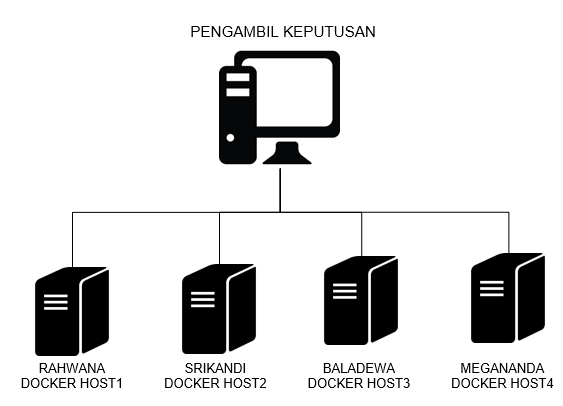
\includegraphics[width=\linewidth]{images/bab5/arsitekturujicoba}
        \caption{Arsitektur Pengujian Performa}
        \label{skenarioSkalabilitas}
      \end{figure} 
    \section{Hasil Uji Coba dan Evaluasi}
    	Berikut dijelaskan hasil uji coba dan evaluasi berdasarkan skenario yang sudah dijelaskan pada bab 5.2.

\subsection{Uji Fungsionalitas}
Berikut dijelaskan hasil pengujian fungsionalitas pada sistem.
\subsubsection{Uji Coba User Mengirim Permintaan Penyediaan Kontainer}
      Uji coba ini dilakukan dengan mengakses sistem melalui rute dan parameter yang telah ditentukan pada Tabel \ref{sUF1}. Pengguna akan mengirim \textit{http request} kepada web service yang telah disediakan pada Komputer Penerima Permintaan Penyediaan Kontainer. Hasil uji coba seperti tertera pada tabel \ref{HsUF1}.
      
      \begin{longtable}{|p{0.03\textwidth}|p{0.25\textwidth}|p{0.21\textwidth}|p{0.35\textwidth}|} % L = Rata kiri untuk setiap kolom, | = garis batas vertikal.

% Kepala tabel, berulang di setiap halaman
\caption{Hasil Skenario Uji Coba mengirim permintaan penyediaan kontainer} \label{HsUF1} \\
\hline
\textbf{No} & \textbf{Routes} & \textbf{Uji Coba} & \textbf{Hasil} \\ \hline
\endfirsthead
\caption[]{Hasil Skenario uji Coba mengirim permintaan penyediaan kontainer}  \\
\hline
\textbf{No} & \textbf{Routes} & \textbf{Uji Coba} & \textbf{Hasil} \\ \hline
\endhead
\endfoot
\endlastfoot
% Isi Tabel
1 & /data/httpd & Mengirim request menuju rute web service melalui browser. & OK. \\ \hline
\end{longtable}	

\subsubsection{Uji Coba Sistem dapat Melakukan Penghitungan AHP}
      Uji coba ini dilakukan dengan mengakses sistem melalui rute yang telah ditentukan pada Tabel \ref{sUF2}. Pengguna akan mengirim \textit{http request} kepada web service yang telah disediakan pada Komputer Penerima Permintaan Penyediaan Kontainer dan sistem akan melakukan penghitungan AHP terhadap data sumber daya setiap \textit{docker host} yang ada sebagai acuan. Hasil uji coba seperti tertera pada Tabel \ref{ujif1.1} dan \ref{ujif1}.
     

\begin{longtable}{|p{0.11\textwidth}|p{0.20\textwidth}|p{0.15\textwidth}|p{0.17\textwidth}|p{0.19\textwidth}|} % L = Rata kiri untuk setiap kolom, | = garis batas vertikal.

% Kepala tabel, berulang di setiap halaman
\caption{Kondisi Awal Penggunaan Sumberdaya \textit{Docker Host} sebelum uji coba dijalankan} \label{ujif1.1} \\
\hline
\textbf{No} & \textbf{Docker Host} & \textbf{CPU} & \textbf{RAM}  & \textbf{Storage} \\ \hline
\endfirsthead
\caption[]{Kondisi Awal Penggunaan Sumberdaya \textit{Docker Host} sebelum uji coba dijalankan}  \\
\hline
\textbf{No} & \textbf{Docker Host} & \textbf{CPU} & \textbf{RAM} & \textbf{Storage} \\ \hline
\endhead
\endfoot
\endlastfoot

% Isi Tabel
1 & RAHWANA & 0.2\%  & 797M/1.9G & 11G/16G \\ \hline
2 & SRIKANDI & 0.3\%  & 532M/2.9G & 8.8G/50G \\ \hline
3 & BALADEWA & 0.1\%  & 354M1.9G/ & 37G/57G \\ \hline
4 & MEGANANDA & 0.1\%  & 555M/1.9G & 10G/16G \\ \hline
\end{longtable}

\begin{longtable}{|p{0.03\textwidth}|p{0.25\textwidth}|p{0.21\textwidth}|p{0.35\textwidth}|} % L = Rata kiri untuk setiap kolom, | = garis batas vertikal.

% Kepala tabel, berulang di setiap halaman
\caption{Hasil Skenario Uji Coba Sistem dapat melakukan Penghitungan AHP} \label{ujif1} \\
\hline
\textbf{No} & \textbf{Docker Host} & \textbf{Uji Coba} & \textbf{Hasil} \\ \hline
\endfirsthead
\caption[]{Hasil Skenario Uji Coba Sistem dapat melakukan Penghitungan AHP}  \\
\hline
\textbf{No} & \textbf{Routes} & \textbf{Uji Coba} & \textbf{Hasil} \\ \hline
\endhead
\endfoot
\endlastfoot
% Isi Tabel
1 & /data/httpd & Mengirim request menuju rute web service melalui browser. & web service berhasil melakukan AHP dan menghasilkan hostname dari \textit{docker host} terpilih, yaitu dalam uji coba ini menghasilkan \textit{hostname} SRIKANDI. \\ \hline
\end{longtable}	

Pada Uji Coba berhasil didapatkan hostname dari \textit{Docker Host} terbaik, yaitu SRIKANDI seperti yang ditunjukkan pada Gambar \ref{gambarujif1}, dikarenakan SRIKANDI memiliki ketersediaan sumber daya yang lebih baik dibanding \textit{Docker Host} lain berdasarkan penghitungan dengan menggunakan algortima AHP.

\begin{figure}[H]
\centering
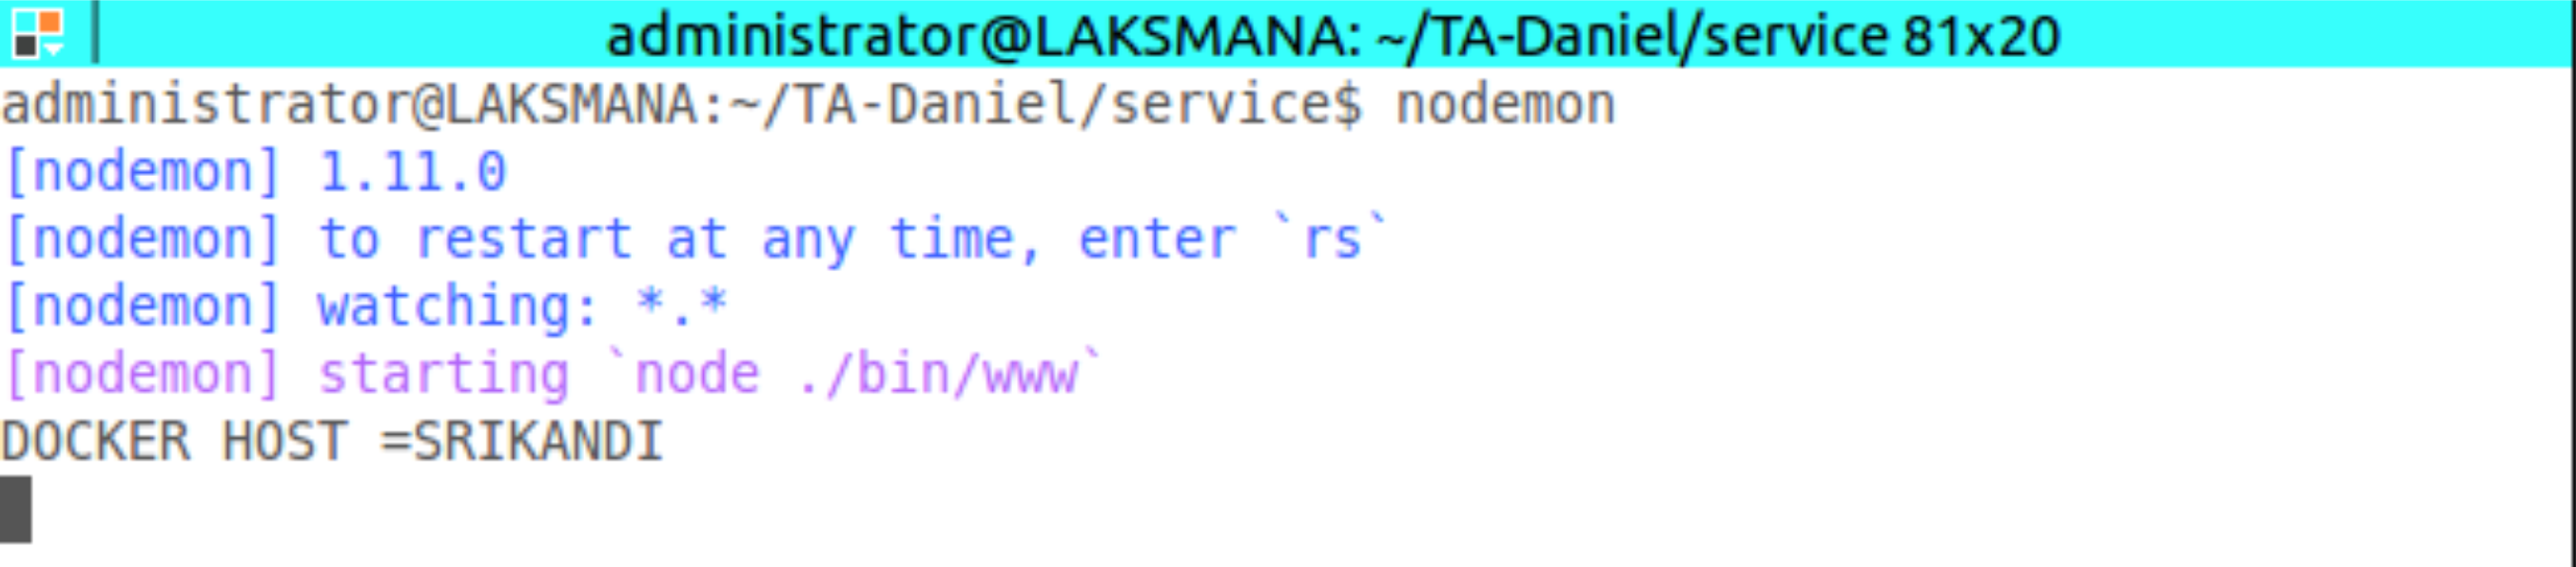
\includegraphics[width=\linewidth]{images/bab5/Selection_005}
\caption{Gambar Hasil Uji Sistem dapat melakukan Penghitungan AHP }
\label{gambarujif1}
\end{figure}     


\subsubsection{Uji Coba \textit{Docker Host} dapat Menerima Perintah Penyediaan Kontainer}
      Uji coba ini dilakukan dengan mengakses sistem melalui rute, parameter  yang telah ditentukan pada Tabel \ref{sUF3}. Pengujian dilakukan image httpd yang akan diujikan pada setiap \textit{docker host}. Hasil uji coba ditunjukkan pada Tabel \ref{Hsuf3}
      
      \begin{longtable}{|p{0.11\textwidth}|p{0.20\textwidth}|p{0.15\textwidth}|p{0.17\textwidth}|p{0.19\textwidth}|} % L = Rata kiri untuk setiap kolom, | = garis batas vertikal.

% Kepala tabel, berulang di setiap halaman
\caption{Hasil Skenario Uji Coba \textit{Docker Host} dapat menerima perintah penyediaan kontainer} \label{Hsuf3} \\
\hline
\textbf{No} & \textbf{Route} & \textbf{Docker Host} & \textbf{Uji Coba} & \textbf{Hasil} \\ \hline
\endfirsthead
\caption[]{Hasil Skenario Uji Coba \textit{Docker Host} dapat menerima perintah penyediaan kontainer}  \\
\hline
\textbf{No} & \textbf{Route} & \textbf{Docker Host} & \textbf{Uji Coba} & \textbf{Hasil} \\ \hline
\endhead
\endfoot
\endlastfoot

% Isi Tabel
1 & /data/httpd & \textit{Docker Host} 1 & Mengirim request penyediaan \textit{docker} dengan image httpd menuju rute web service melalui browser. & \textit{Docker Host} berhasil menerima perintah penyediaan kontainer dan menyediakan kontainer \textit{docker} dengan image httpd. \\ \hline
2 & /data/httpd & \textit{Docker Host} 2 & Mengirim request penyediaan \textit{docker} dengan image httpd menuju rute web service melalui browser. & \textit{Docker Host} berhasil menerima perintah penyediaan kontainer dan menyediakan kontainer \textit{docker} dengan image httpd. \\ \hline
3 & /data/httpd & \textit{Docker Host} 3 & Mengirim request penyediaan \textit{docker} dengan image httpd menuju rute web service melalui browser. & \textit{Docker Host} berhasil menerima perintah penyediaan kontainer dan menyediakan kontainer \textit{docker} dengan image httpd. \\ \hline
4 & /data/httpd & \textit{Docker Host} 4 & Mengirim request penyediaan \textit{docker} dengan image httpd menuju rute web service melalui browser. & \textit{Docker Host} berhasil menerima perintah penyediaan kontainer dan menyediakan kontainer \textit{docker} dengan image httpd. \\ \hline
\end{longtable}
Pada Gambar \ref{perintahansible} dan Gambar \ref{dockerterpasang} ditunjukkan bagaimana kondisi saat sistem menghasilkan perintah untuk menyediakan \textit{docker} dan saat \textit{docker} sudah terpasang pada \textit{docker host}

\begin{figure}[H]
\centering
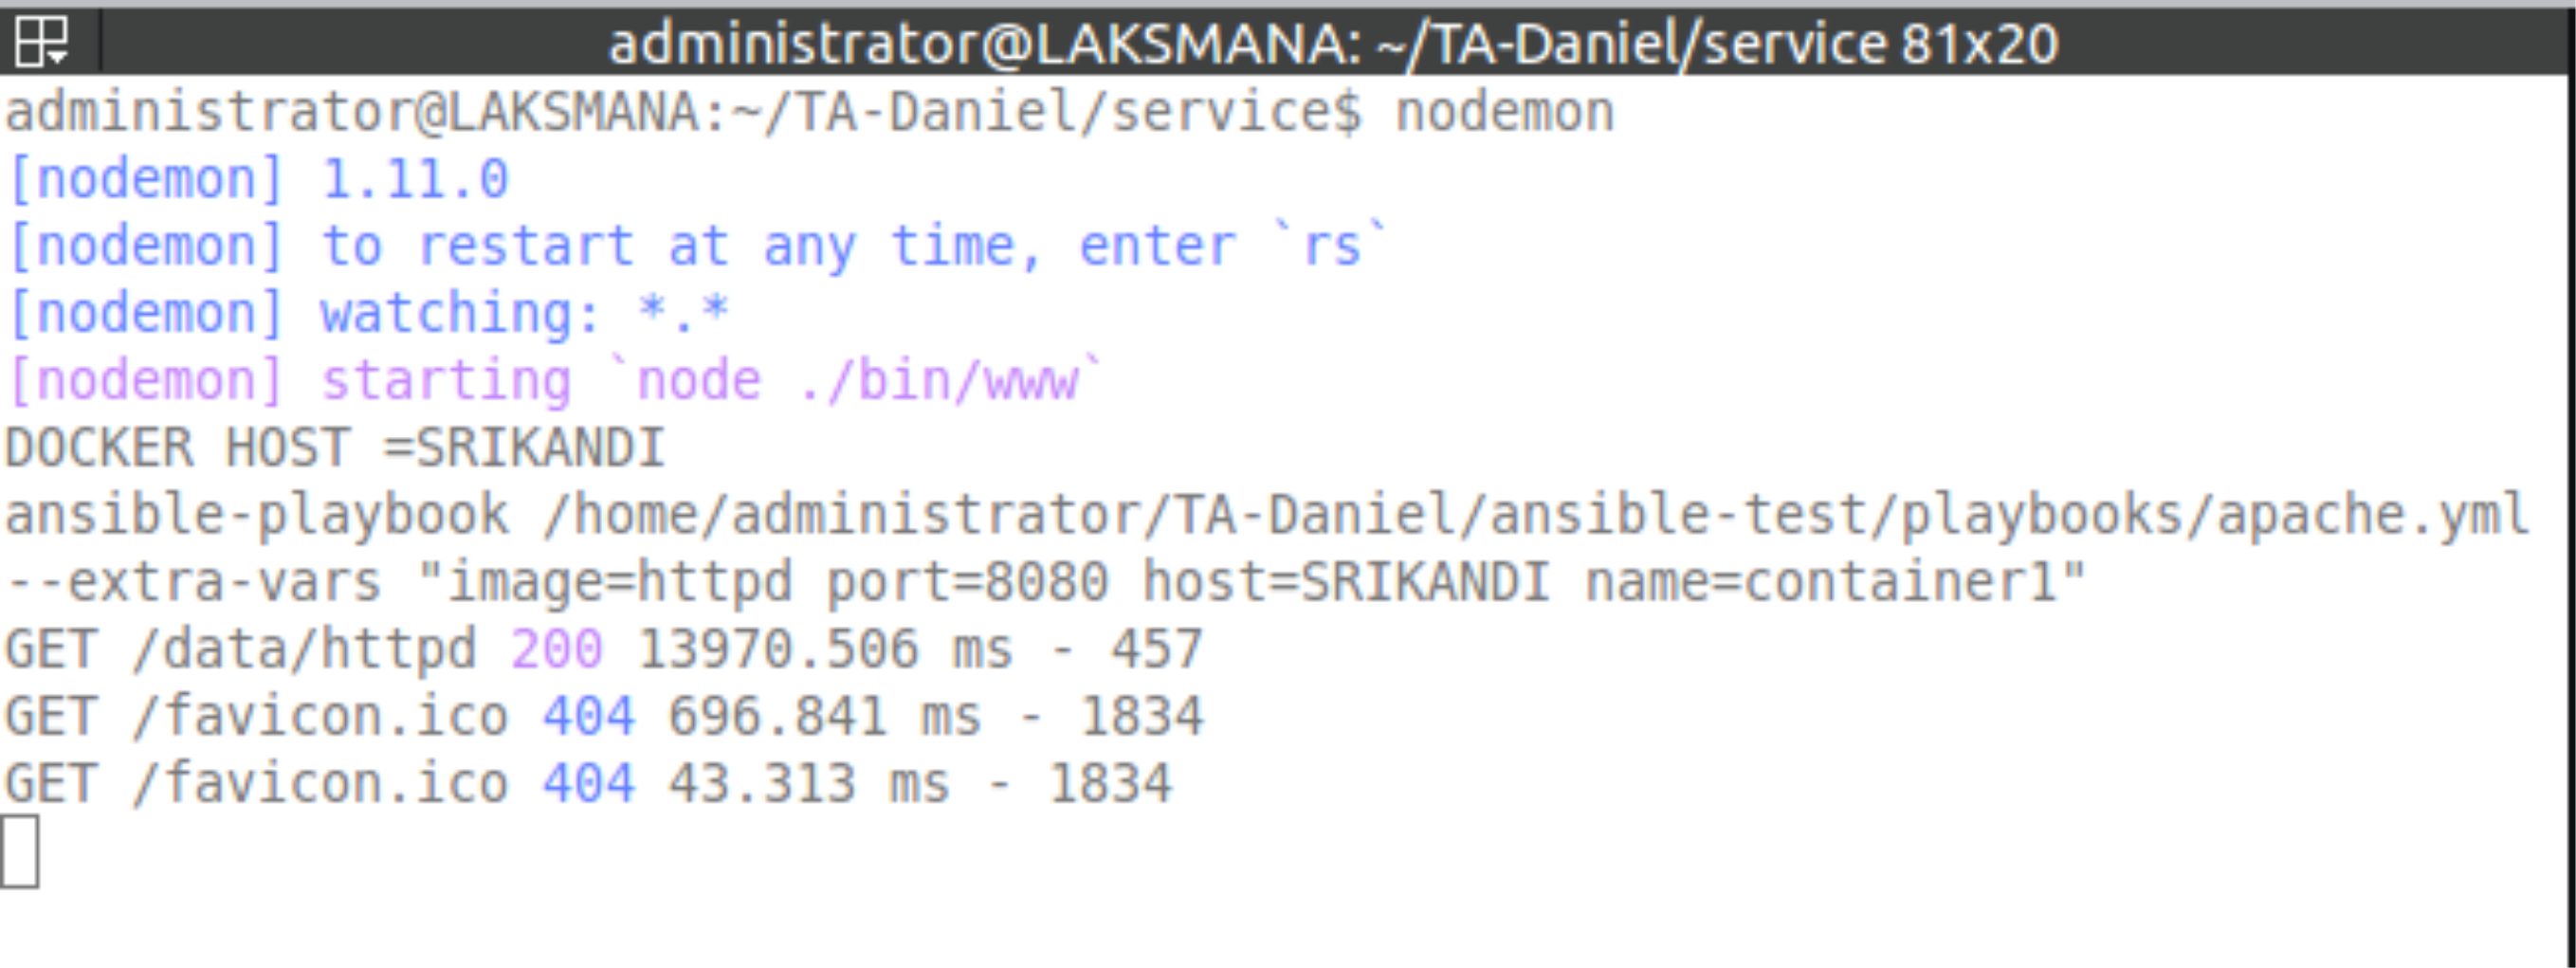
\includegraphics[width=\linewidth]{images/bab5/Selection_006}
\caption{Web Service Mengrimkan perintah penyediaan kontainer}
\label{perintahansible}
\end{figure}     

\begin{figure}[H]
\centering
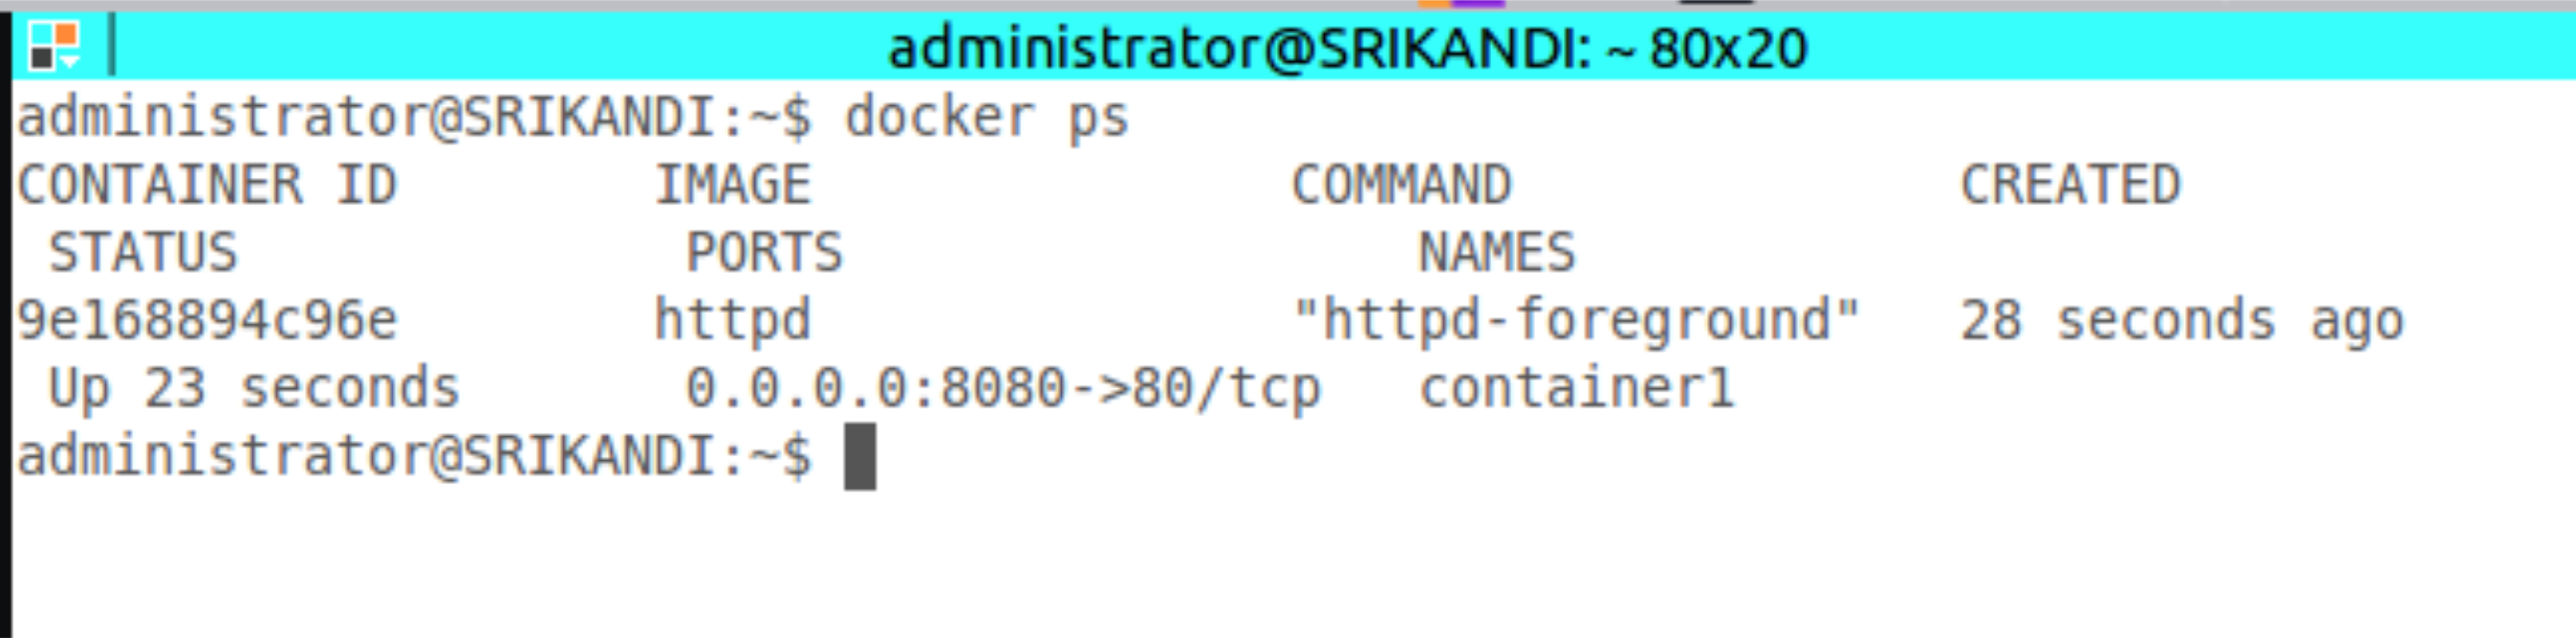
\includegraphics[width=\linewidth]{images/bab5/Selection_007}
\caption{\emph{Docker Host} berhasil membuat kontainer \emph{docker}}
\label{dockerterpasang}
\end{figure}     

\subsubsection{Uji Coba \textit{Docker Host} dapat Mengirim Data Resourcenya Masing-Masing}
      Dilakukan pengujian pada setiap \textit{docker host}. Setiap \textit{docker host} akan mengirimkan data ketersediaan sumber daya CPU, RAM dan File Storage nya masing-masing ke InfluxDB yang terdapat pada \textit{middleware}. Hasil ditunjukkan pada Tabel \ref{HsUF4} 
      
      \begin{longtable}{|p{0.03\textwidth}|p{0.25\textwidth}|p{0.21\textwidth}|p{0.35\textwidth}|} % L = Rata kiri untuk setiap kolom, | = garis batas vertikal.

% Kepala tabel, berulang di setiap halaman
\caption{Hasil Skenario Uji Coba \textit{Docker Host} dapat Mengirim Data Resourcenya Masing-Masing} \label{HsUF4} \\
\hline
\textbf{No} & \textbf{Docker Host} & \textbf{Uji Coba} & \textbf{Hasil } \\ \hline
\endfirsthead
\caption[]{Hasil Skenario uji Coba \textit{Docker Host} dapat Mengirim Data Resource}  \\
\hline
\textbf{No} & \textbf{Docker Host} & \textbf{Uji Coba} & \textbf{Hasil } \\ \hline
\endhead
\endfoot
\endlastfoot
% Isi Tabel
1 & \textit{Docker Host} 1 & Mengirim data sumber daya (RAM, CPU dan \textit{File Storage}) ke InfluxDB pada \textit{middleware} . & Data sumber daya CPU, RAM dan File Storage berhasilkan dikirimkan dan tersimpan pada InfluxDB. \\ \hline
2 & \textit{Docker Host} 2 & Mengirim data sumber daya (RAM, CPU dan \textit{File Storage}) ke InfluxDB pada \textit{middleware} . & Data sumber daya CPU, RAM dan File Storage berhasilkan dikirimkan dan tersimpan pada InfluxDB. \\ \hline
3 & \textit{Docker Host} 3 & Mengirim data sumber daya (RAM, CPU dan \textit{File Storage}) ke InfluxDB pada \textit{middleware} . & Data sumber daya CPU, RAM dan File Storage berhasilkan dikirimkan dan tersimpan pada InfluxDB. \\ \hline
4 & \textit{Docker Host} 4 & Mengirim data sumber daya (RAM, CPU dan \textit{File Storage}) ke InfluxDB pada \textit{middleware} . & Data sumber daya CPU, RAM dan File Storage berhasilkan dikirimkan dan tersimpan pada InfluxDB. \\ \hline
\end{longtable}	      
Sesuai dengan Gambar \ref{DataCpu},\ref{DataRam} dan \ref{DataDf}, ,semua \textit{docker host} berhasil mengirimkan data sumber daya CPU, RAM dan File Storage nya masing-masing ke InfluxDB.
\begin{itemize}
\item Data CPU Setiap Docker Host pada InfluxDB
\begin{figure}[H]
        \centering
        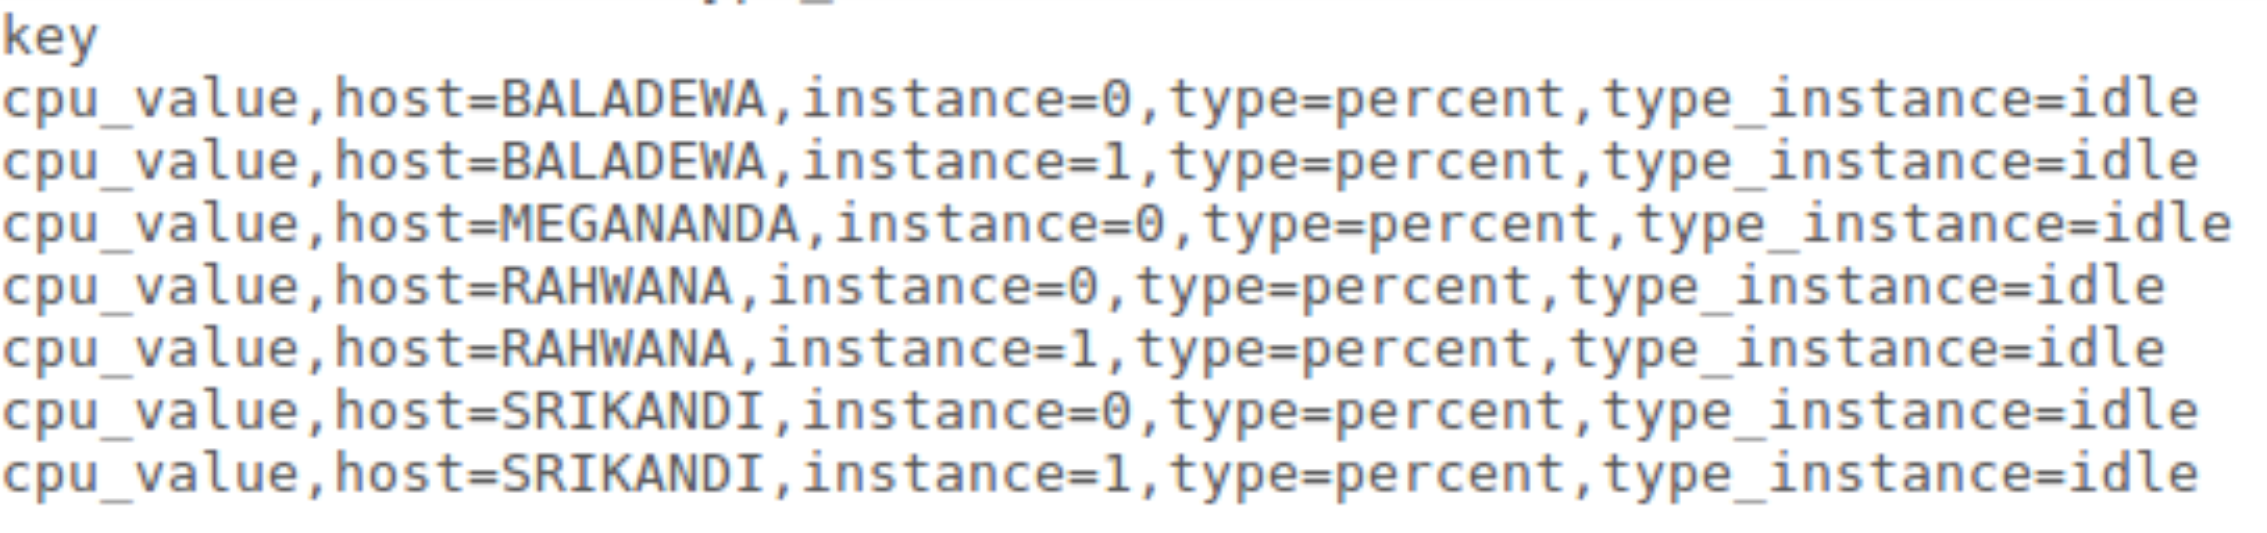
\includegraphics[width=\linewidth]{images/bab5/datacpu}
        \caption{Data CPU Setiap Docker Host pada InfluxDB}
        \label{DataCpu}
      \end{figure} 
\end{itemize}
\begin{itemize}
\item Data RAM Setiap Docker Host pada InfluxDB
\begin{figure}[H]
        \centering
        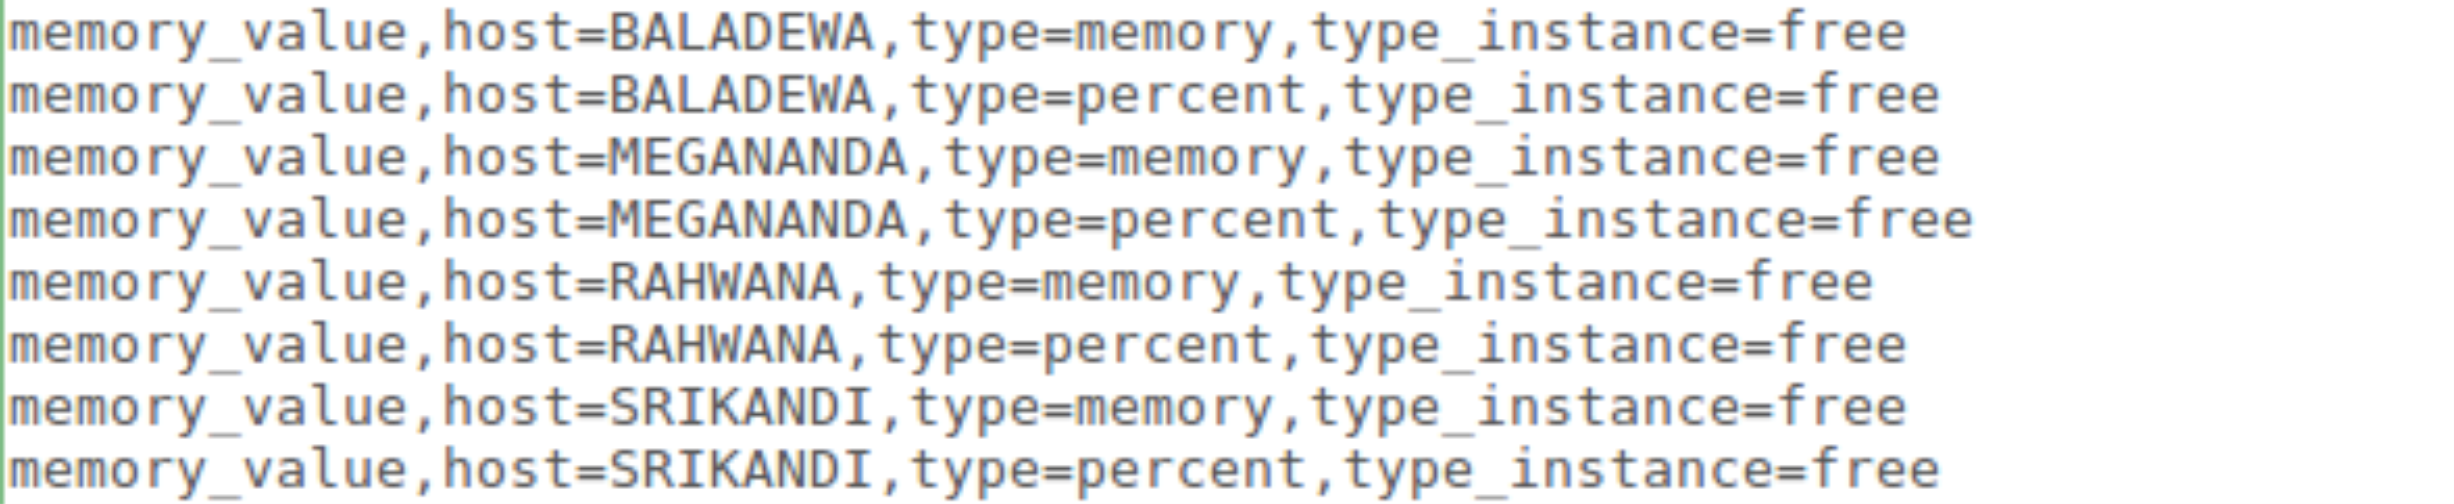
\includegraphics[width=\linewidth]{images/bab5/dataram}
        \caption{Data RAM Setiap Docker Host pada InfluxDB}
        \label{DataRam}
      \end{figure} 
\end{itemize}
\begin{itemize}
\item Data Penyimpanan File Setiap Docker Host pada InfluxDB
\begin{figure}[H]
        \centering
        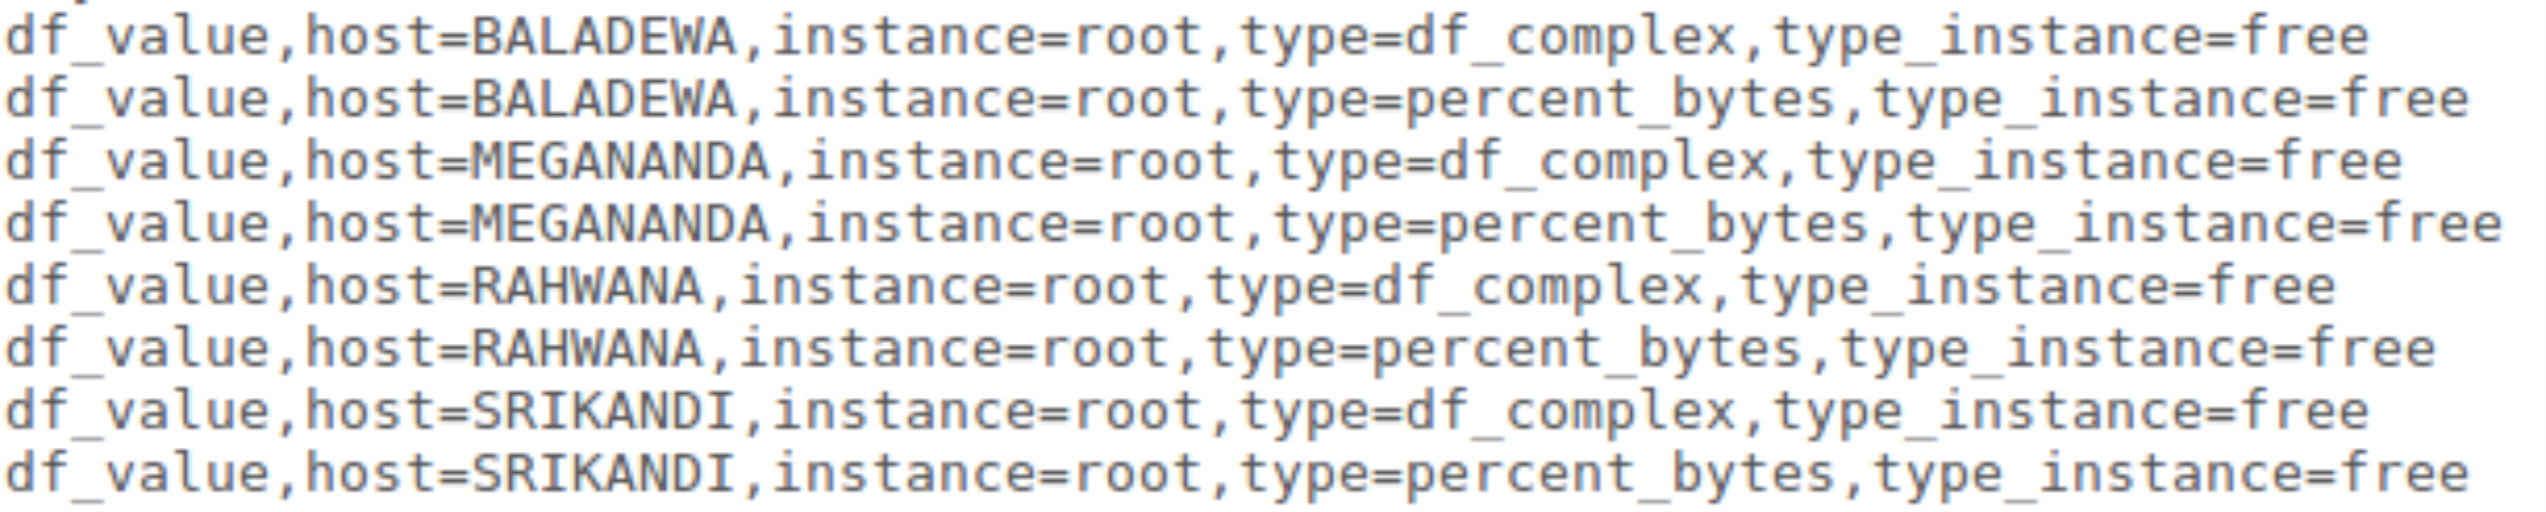
\includegraphics[width=\linewidth]{images/bab5/datadf}
        \caption{Data Penyimpanan File Setiap Docker Host pada InfluxDB}
        \label{DataDf}
      \end{figure} 
\end{itemize}


      \subsection{Uji Performa}
 Seperti yang dijelaskan pada bab 5.2 pengujian performa akan dilakukan pada 4 \textit{docker host} yang tersedia dengan menggunakan sistem yang ada, namun dengan 2 algoritma yang berbeda yaitu menggunakan algoritma pengambilan keputusan AHP dan menggunakan algoritma pembagian kerja dasar, \textit{round robin}[xx]. Selain itu pengujian juga akan menggunakan beberapa image \textit{docker} yang akan di pasangkan pada setiap \textit{docker host} yang tersedia. Pengujian akan dijalankan dengan mengirimkan permintaan penyediaan kontainer pada sistem dengan jumlah permintaan penyediaan kontainer yang beragam.

\subsubsection{Pengujian Dengan Algoritma AHP}
Kondisi awal ketersediaan sumberdaya \textit{docker host} sebelum uji coba sistem dengan image \textit{docker} httpd dan nginx menggunakan AHP dijalankan ditunjukkan pada Tabel \ref{kondisiawal1}.
\begin{longtable}{|p{0.08\textwidth}|p{0.24\textwidth}|p{0.15\textwidth}|p{0.17\textwidth}|p{0.19\textwidth}|} % L = Rata kiri untuk setiap kolom, | = garis batas vertikal.

% Kepala tabel, berulang di setiap halaman
\caption{Kondisi Awal Ketersediaan Sumberdaya \textit{Docker Host} sebelum uji coba dijalankan} \label{kondisiawal1} \\
\hline
\textbf{No} & \textbf{Docker Host} & \textbf{CPU} & \textbf{RAM}  & \textbf{Storage} \\ \hline
\endfirsthead
\caption[]{Kondisi Awal Ketersediaan Sumberdaya \textit{Docker Host} Sebelum Uji Coba Dijalankan}  \\
\hline
\textbf{No} & \textbf{Docker Host} & \textbf{CPU} & \textbf{RAM} & \textbf{Storage} \\ \hline
\endhead
\endfoot
\endlastfoot

% Isi Tabel
1 & RAHWANA & 98\%  & 1.3G/1.9G & 5G/16G \\ \hline
2 & SRIKANDI & 93\%  & 2.3G/2.9G & 41.2G/50G \\ \hline
3 & BALADEWA & 99\%  & 1G/1.9G & 20G/57G \\ \hline
4 & MEGANANDA & 91\%  & 1.3G/1.9G & 6G/16G \\ \hline
\end{longtable}

Hasil pengujian sistem dengan algoritma AHP menggunakan \textit{image docker} httpd dan nginx ditunjukkan pada Tabel \ref{Uji Performa1}.
\begin{longtable}{|p{0.05\textwidth}|p{0.15\textwidth}|p{0.15\textwidth}|p{0.15\textwidth}|p{0.15\textwidth}|p{0.15\textwidth}|}
\caption{Hasil Uji Coba Performa sistem dengan \textit{Image Docker} httpd dan nginx menggunakan AHP}
\label{Uji Performa1} \\
\hline
\multirow{2}{*}{No} & \multirow{2}{*}{\begin{tabular}[c]{@{}c@{}}Jumlah\\ Kontainer\end{tabular}} & \multicolumn{4}{c|}{Kontainer Terpasang pada \textit{Docker Host}} \\ \cline{3-6} 
  & 	& Rahwana  & Srikandi  & Baladewa & Megananda    \\ \hline
1 & 254 & 39       & 135       & 27       & 53       \\ \hline
2 & 254 & 40       & 131       & 32       & 51       \\ \hline
3 & 254 & 37       & 147       & 20       & 50       \\ \hline
4 & 254 & 41       & 143       & 23       & 47       \\ \hline
5 & 254 & 49       & 132       & 24       & 49       \\ \hline
\end{longtable}  

Kondisi akhir  ketersediaan sumber daya \textit{docker host} pada pengujian sistem dengan algoritma AHP menggunakan \textit{image docker} httpd dan nginx ditunjukkan pada Tabel \ref{kondisiakhir1}.
\begin{longtable}{|p{0.08\textwidth}|p{0.24\textwidth}|p{0.15\textwidth}|p{0.17\textwidth}|p{0.19\textwidth}|} % L = Rata kiri untuk setiap kolom, | = garis batas vertikal.

% Kepala tabel, berulang di setiap halaman
\caption{Rata-rata Kondisi Akhir Ketersediaan Sumberdaya \textit{Docker Host} Setelah Uji Coba Dijalankan} \label{kondisiakhir1} \\
\hline
\textbf{No} & \textbf{Docker Host} & \textbf{CPU} & \textbf{RAM}  & \textbf{Storage} \\ \hline
\endfirsthead
\caption[]{Rata-rata Kondisi Akhir Ketersediaan Sumberdaya \textit{Docker Host} Setelah Uji Coba Dijalankan}  \\
\hline
\textbf{No} & \textbf{Docker Host} & \textbf{CPU} & \textbf{RAM} & \textbf{Storage} \\ \hline
\endhead
\endfoot
\endlastfoot

% Isi Tabel
1 & RAHWANA & 90\%  & 628M/1.9G & 5G/16G \\ \hline
2 & SRIKANDI & 85\%  & 708M/2.9G & 41.2G/50G \\ \hline
3 & BALADEWA & 92\%  & 832M/1.9G & 20G/57G \\ \hline
4 & MEGANANDA & 90\%  & 654M/1.9G & 6G/16G \\ \hline
\end{longtable}

\subsubsection{Pengujian Dengan Algoritma \textit{Round Robin}}
Kondisi awal ketersediaan sumberdaya \textit{docker host} sebelum uji coba sistem dengan \textit{image docker} httpd dan nginx menggunakan \textit{round robin} dijalankan ditunjukkan pada Tabel \ref{kondisiawal2}.
\begin{longtable}{|p{0.08\textwidth}|p{0.24\textwidth}|p{0.15\textwidth}|p{0.17\textwidth}|p{0.19\textwidth}|} % L = Rata kiri untuk setiap kolom, | = garis batas vertikal.

% Kepala tabel, berulang di setiap halaman
\caption{Kondisi Awal Ketersediaan Sumberdaya \textit{Docker Host} Sebelum Uji Coba Dijalankan} \label{kondisiawal2} \\
\hline
\textbf{No} & \textbf{Docker Host} & \textbf{CPU} & \textbf{RAM}  & \textbf{Storage} \\ \hline
\endfirsthead
\caption[]{Kondisi Awal Ketersediaan Sumberdaya \textit{Docker Host} Sebelum Uji Coba Dijalankan}  \\
\hline
\textbf{No} & \textbf{Docker Host} & \textbf{CPU} & \textbf{RAM} & \textbf{Storage} \\ \hline
\endhead
\endfoot
\endlastfoot

% Isi Tabel
1 & RAHWANA & 98\%  & 1.2G/1.9G & 5G/16G \\ \hline
2 & SRIKANDI & 93\%  & 2.3G/2.9G & 41.2G/50G \\ \hline
3 & BALADEWA & 99\%  & 1G/1.9G & 20G/57G \\ \hline
4 & MEGANANDA & 91\%  & 1.4G/1.9G & 6G/16G \\ \hline
\end{longtable}

Hasil dari pengujian sistem dengan algoritma \textit{round robin} ditunjukkan pada Tabel \ref{Uji Performa2}.
\begin{longtable}{|p{0.05\textwidth}|p{0.15\textwidth}|p{0.15\textwidth}|p{0.15
\textwidth}|p{0.15\textwidth}|p{0.15\textwidth}|}
\caption{Hasil Uji Coba Performa Sistem dengan \textit{Image Docker} httpd dan nginx Menggunakan \textit{Round Robin}}
\label{Uji Performa2} \\
\hline
\multirow{2}{*}{No} & \multirow{2}{*}{\begin{tabular}[c]{@{}c@{}}Jumlah\\ Kontainer\end{tabular}} & \multicolumn{4}{c|}{Kontainer Terpasang pada Docker Host} \\ \cline{3-6} 
  &		& Rahwana  & Srikandi & Baladewa & Megananda    \\ \hline
1 & 254 & 63       & 63       & 63       & 63       \\ \hline
2 & 254 & 63       & 63       & 63       & 63       \\ \hline
3 & 254 & 63       & 63       & 63       & 63       \\ \hline
4 & 254 & 63       & 63       & 63       & 63       \\ \hline
5 & 254 & 63       & 63       & 63       & 63       \\ \hline
\end{longtable}
Kondisi akhir ketersediaan sumberdaya \textit{docker host} pada pengujian sistem dengan algoritma \textit{round robin} menggunakan \textit{image docker} httpd dan nginx ditunjukkan pada Tabel \ref{kondisiakhir2}.
\begin{longtable}{|p{0.08\textwidth}|p{0.22\textwidth}|p{0.15\textwidth}|p{0.17\textwidth}|p{0.19\textwidth}|} % L = Rata kiri untuk setiap kolom, | = garis batas vertikal.

% Kepala tabel, berulang di setiap halaman
\caption{Kondisi Akhir Ketersediaan Sumberdaya \textit{Docker Host} Setelah Uji Coba Dijalankan} \label{kondisiakhir2} \\
\hline
\textbf{No} & \textbf{Docker Host} & \textbf{CPU} & \textbf{RAM}  & \textbf{Storage} \\ \hline
\endfirsthead
\caption[]{Kondisi Akhir Ketersediaan Sumberdaya \textit{Docker Host} Setelah Uji Coba Dijalankan}  \\
\hline
\textbf{No} & \textbf{Docker Host} & \textbf{CPU} & \textbf{RAM} & \textbf{Storage} \\ \hline
\endhead
\endfoot
\endlastfoot

% Isi Tabel
1 & RAHWANA & 92\%  & 161M/1.9G & 5G/16G \\ \hline
2 & SRIKANDI & 93\%  & 1.3G/2.9G & 41.1G/50G \\ \hline
3 & BALADEWA & 92\%  & 95M/1.9G & 20G/57G \\ \hline
4 & MEGANANDA & 91\%  & 335M/1.9G & 6G/16G \\ \hline
\end{longtable}  

\subsubsection{Pengujian Performa Sistem dengan Algoritma AHP Berdasarkan Jumlah Kontainer yang Akan Dipasangkan}
Kondisi awal ketersediaan sumberdaya \textit{docker host} sebelum uji coba ditunjukkan pada Tabel \ref{kondisiawal3}.
\begin{longtable}{|p{0.08\textwidth}|p{0.24\textwidth}|p{0.15\textwidth}|p{0.17\textwidth}|p{0.19\textwidth}|} % L = Rata kiri untuk setiap kolom, | = garis batas vertikal.

% Kepala tabel, berulang di setiap halaman
\caption{Kondisi Awal Ketersediaan Sumberdaya \textit{Docker Host} Sebelum Uji Coba Dijalankan} \label{kondisiawal3} \\
\hline
\textbf{No} & \textbf{Docker Host} & \textbf{CPU} & \textbf{RAM}  & \textbf{Storage} \\ \hline
\endfirsthead
\caption[]{Kondisi Awal Ketersediaan Sumberdaya \textit{Docker Host} Sebelum Uji Coba Dijalankan}  \\
\hline
\textbf{No} & \textbf{Docker Host} & \textbf{CPU} & \textbf{RAM} & \textbf{Storage} \\ \hline
\endhead
\endfoot
\endlastfoot

% Isi Tabel
1 & RAHWANA & 99\%  & 1.3G/1.9G & 3.8G/16G \\ \hline
2 & SRIKANDI & 99\%  & 2.3G/2.9G & 37G/50G \\ \hline
3 & BALADEWA & 99\%  & 1G/1.9G & 16G/57G \\ \hline
4 & MEGANANDA & 99\%  & 1.4G/1.9G & 3.8G/16G \\ \hline
\end{longtable}
Hasil pengujian sistem dengan algoritma AHP menggunakan \textit{docker image} httpd, nginx, moodle, dan mysql ditunjukkan pada Table \ref{Uji Performa3}.
\begin{longtable}{|p{0.05\textwidth}|p{0.15\textwidth}|p{0.15\textwidth}|p{0.15\textwidth}|p{0.15\textwidth}|p{0.15\textwidth}|}
\caption{Hasil Uji Coba Performa Sistem dengan \textit{Docker Image} httpd dan nginx Menggunakan AHP}
\label{Uji Performa3} \\
\hline
\multirow{2}{*}{No} & \multirow{2}{*}{\begin{tabular}[c]{@{}c@{}}Jumlah\\ Kontainer\end{tabular}} & \multicolumn{4}{c|}{Kontainer Terpasang pada Docker Host} \\ \cline{3-6} 
  &	 	& Rahwana   & Srikandi & Baladewa & Megananda    \\ \hline
1 & 30  & 0       	& 30       & 0        & 0       \\ \hline
2 & 60 	& 3       	& 55       & 0        & 2       \\ \hline
3 & 100 & 5       	& 73       & 0        & 12       \\ \hline
4 & 120 & 11       	& 88       & 5        & 16       \\ \hline
5 & 150 & 34       	& 46       & 33       & 37       \\ \hline
\end{longtable} 
Kondisi akhir ketersediaan sumberdaya \textit{docker host} setelah uji coba dijalankan ditunjukkan pada Gambar \ref{Grafik CPU RAHWANA} untuk ketersediaan CPU, Gambar \ref{Grafik RAM RAHWANA} untuk ketersediaan Memori dan Gambar \ref{Grafik DF RAHWANA} untuk ketersediaan penyimpaan berkas. 
\begin{figure}[H]
        \centering
        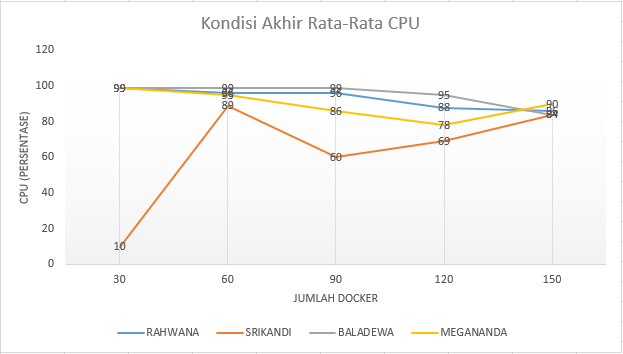
\includegraphics[width=\linewidth]{images/bab5/cpu}
        \caption{Grafik Kondisi Akhir Ketersediaan Rata-Rata CPU}
        \label{Grafik CPU RAHWANA}
      \end{figure} 
\begin{figure}[H]
        \centering
        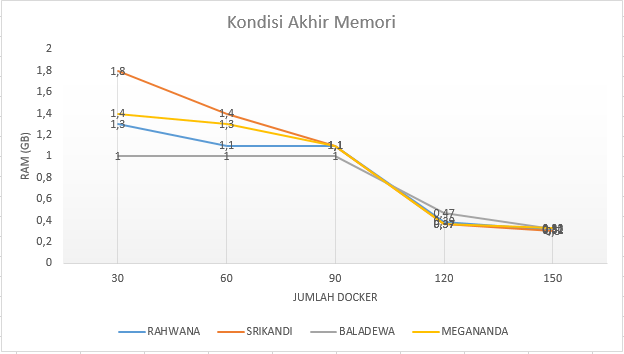
\includegraphics[width=\linewidth]{images/bab5/memori}
        \caption{Grafik Kondisi Akhir Ketersediaan Memori}
        \label{Grafik RAM RAHWANA}
      \end{figure} 
\begin{figure}[H]
        \centering
        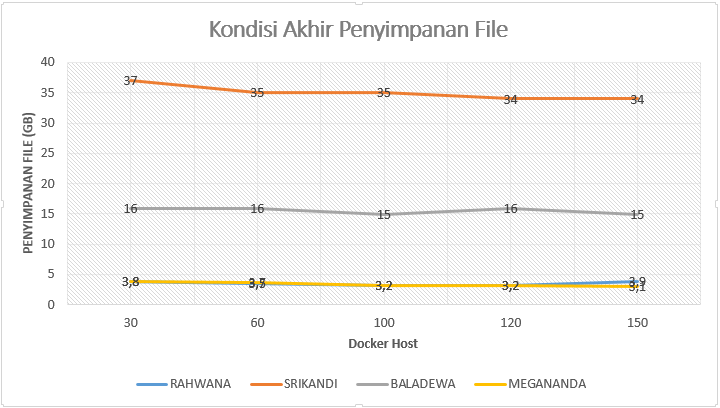
\includegraphics[width=\linewidth]{images/bab5/Storage}
        \caption{Grafik Kondisi Akhir Ketersedian Penyimpaanan FIle}
        \label{Grafik DF RAHWANA}
      \end{figure} 

Waktu Pendistribusian Docker oleh Sistem Berdasarkan Jumlah Kontainer ditunjukkan pada Gambar \ref{Grafik Waktu}
\begin{figure}[H]
        \centering
        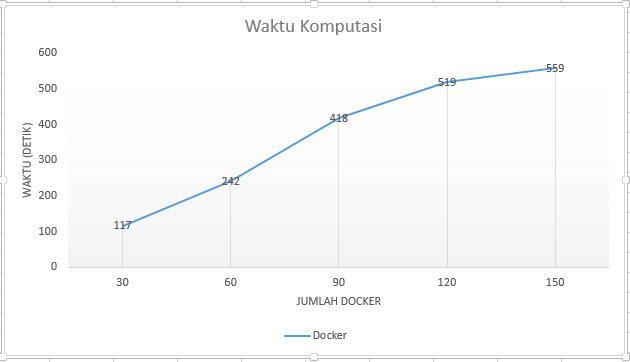
\includegraphics[width=\linewidth]{images/bab5/waktu}
        \caption{Grafik Waktu Pendistribusian Docker oleh Sistem Berdasarkan Jumlah Kontainer}
        \label{Grafik Waktu}
      \end{figure} 

	Dari data hasil uji coba yang didapat, dapat dilihat bahwa algoritma AHP dapat membagikan kontainer ke \textit{docker host} yang ada dengan lebih efisien. Dibandingkan dengan algoritma \textit{round robin} yang menyebarkan kontainer merata ke setiap \textit{docker host}, sistem dengan AHP menghasilkan kondisi ketersediaan sumber daya yang lebih merata pada akhir uji coba. Selain itu pendistribusian pada setiap \textit{docker host} juga memiliki ketepatan yang baik, hal ini terlihat pada saat akan mendistribusikan 30 kontainer, sistem dengan AHP mendistribusikan seluruh kontainer tersebut pada \textit{docker host} SRIKANDI, hal ini disebabkan SRIKANDI memiliki ketersediaan yang jauh lebih dominan dibanding \textit{docker host} yang lain.  Namun, kondisi dimana \textit{docker image} yang bervariasi menimbulkan hasil akhir dari uji coba tidak linear, hal ini disebabkan variasi dari \textit{docker image} akan membuat kebutuhan sumber daya yang dibutuhkan dari setiap \textit{docker host} juga bervariasi.

    % \section{Struktur Dokumen \LaTeX{}}
% Dokumen \LaTeX{} terdiri dari struktur yang dibuat berdasarkan struktur dokumen sehari-hari. Sebagai penulis dokumen, Anda wajib menggunakan struktur ini sehingga \LaTeX{} dapat melakukan hal lain yang membantu Anda dalam mengorganisir dokumen seperti misalnya pembuatan Daftar Isi. Berikut adalah struktur dokumen yang ada di \LaTeX{} diurutkan berdasarkan hirarkinya.

% \begin{ltabulary}{|L|L|} % L = Rata kiri untuk setiap kolom, | = garis batas vertikal.

% % Kepala tabel, berulang di setiap halaman
% \caption{Struktur hirarki dokumen \LaTeX{}} \label{tabelStrukturDokumen} \\
% \hline
% \textbf{Nama} & \textbf{Peruntukkan} \\ \hline

% \endhead
% \endfoot
% \endlastfoot

% % Isi Tabel
% \textbf{\textbackslash{}part\{Judul Bagian\}} & \texttt{book} \\ \hline
% \textbf{\textbackslash{}chapter\{Judul Bab\}} & \texttt{book} dan \texttt{report} \\ \hline
% \textbf{\textbackslash{}section\{Judul Subbab\}} & semua kecuali \texttt{letter} \\ \hline
% \textbf{\textbackslash{}subsection\{Judul Subsubbab\}} & semua kecuali \texttt{letter} \\ \hline
% \textbf{\textbackslash{}subsubsection\{Judul Subsubsubbab\}} & semua kecuali \texttt{letter} \\ \hline
% \textbf{\textbackslash{}paragraph\{Judul Paragraf\}} & semua\\ \hline

% \end{ltabulary}

    \chapter{PENUTUP}
  Bab ini membahas kesimpulan yang dapat diambil dari tujuan pembuatan sistem dan hubungannya dengan hasil uji coba dan evaluasi yang telah dilakukan. Selain itu, terdapat beberapa saran yang bisa dijadikan acuan untuk melakukan pengembangan dan penelitian lebih lanjut.
  \section{Kesimpulan}
  Dari proses perancangan, implementasi dan pengujian terhadap sistem, dapat diambil beberapa kesimpulan berikut:
  \begin{enumerate}
    \item Sistem dapat mendistribusikan 100\% penyediaan kontainer ke \textit{docker host} yang ada dengan multi kriteria dengan cara mendistirbusikan perintah penyediaan kontainer \textit{docker} melalui protokol ssh.  
    \item Sistem dapat menentukan penyedia kontainer dengan menggunakan algoritma AHP dengan kriteria-kriteria seperti penggunaan CPU, RAM , dan Penyimpanan File pada masing-masing \textit{docker host} yang ada.
    \item Dengan menggunakan AHP, dibandingkan dengan metode \textit{round robin}, sistem dapat menentukan \textit{docker host} yang akan menyediakan kontainer docker dengan efisien berdasarkan penggunaan CPU, RAM , dan File Storage pada masing-masing \textit{docker host} yang ada, dimana dengan menggunakan AHP ketersediaan akhir memori dari setiap \textit{docker host} lebih merata dengan rentang 628MB sampai 832MB, sedangkan dengan \textit{round robin} ketersediaan akhir memori sangat tidak merata, dengan rentang yang cukup jauh dimulai 95MB sampai 1.3GB. 
    
  \end{enumerate}
  \section{Saran}
  Berikut beberapa saran yang diberikan untuk pengembangan lebih lanjut:
  \begin{itemize}
    \item Sistem dapat dikembangkan dengan menambahkan kriteria-kriteria yang sesuai dengan lingkungan sistem yang ada, seperti jarak antara \textit{docker host} dan \textit{server} middleware atau kecepatan bandwith dari setiap \textit{docker host} merupakan kriteria yang lebih baik untuk sistem yang memasangkan kontainer yang tidak memiliki perkembangan penggunaan pada aplikasi yang terdapat pada kontainer. Sedangkan sumber daya seperti file storage dapat digunakan untuk sistem yang mengalami perkembangan penggunaan pada aplikasi yang terdapat pada kontainernya.
    \item AHP merupakan algoritma MCDM yang paling umum digunakan dikarenakan proses yang tidak rumit dan memiliki unsur objektif dan subjektif dalam pengambilan keputusannya. Untuk pengembangan kedepannya sistem dapat diimplementasikan dengan menggunakan algortima MCDM lain untuk meningkatkan performa sistem, seperi algoritma Fuzzy AHP.
  \end{itemize}

% Daftar Pustaka
\bibliography{Zotero}
\bibliographystyle{ieeetr}
    \appendix % Halaman lampiran, dengan judul LAMPIRAN X
  	\renewcommand\chaptername{LAMPIRAN}
\chapter{Lampiran Halaman \textit{Login}}
\section{Pemasangan Perangkat Lunak}
\label{lampiranisntalasihalamanlogin}
Berikut adalah perangkat lunak yang dibutuhkan agar halaman \textit{login} dapat digunakan, antara lain:
\begin{enumerate}
	\item \textit{Python} versi 3.5.2.
	\item \textit{Flask} versi 1.0.2.
	\item \textit{Gunicorn} versi 19.8.1.
	\item \textit{Supervisor} versi 3.2.0.
	\item \textit{Nginx} versi 1.10.3.
\end{enumerate}

\subsection{Pemasangan Perangkat Lunak Python}
Berikut adalah langkah-langkah untuk memasang perangkat lunak Python versi 3.5.2 pada \textit{server} yang akan digunakan untuk membangun halaman \textit{login}.\\
\begin{minipage}{\linewidth}
	\begin{lstlisting}[caption=Command untuk installasi Python,language=Python,label=installpython3diserverlogin]
	sudo apt-get update
	sudo apt-get install python3
	\end{lstlisting}
\end{minipage}

\subsection{Pemasangan Perangkat Lunak Flask}
Berikut adalah langkah-langkah untuk memasang perangkat lunak Flask versi 1.0.2 pada \textit{server} yang akan digunakan untuk membangun halaman \textit{login}.\\
\begin{minipage}{\linewidth}
	\begin{lstlisting}[caption=Command untuk installasi Flask,language=Python,label=installflaskdiserverlogin]
	sudo apt-get install python3-pip
	sudo pip install flask
	\end{lstlisting}
\end{minipage}

\subsection{Pemasangan Perangkat Lunak Gunicorn}
Berikut adalah langkah-langkah untuk memasang perangkat lunak Gunicorn versi 19.8.1 pada \textit{server} yang akan digunakan untuk membangun halaman \textit{login}.\\
\begin{minipage}{\linewidth}
 	\begin{lstlisting}[caption=Command untuk installasi Gunicorn,language=Python,label=installgunicorndiserverlogin]
 	sudo pip install gunicorn
 	\end{lstlisting}
\end{minipage}

\subsection{Pemasangan Perangkat Lunak Supervisor}
Berikut adalah langkah-langkah untuk memasang perangkat lunak Supervisor versi 3.2.0 pada \textit{server} yang akan digunakan untuk membangun halaman \textit{login}.\\
\begin{minipage}{\linewidth}
 	\begin{lstlisting}[caption=Command untuk installasi Supervisor,language=Python,label=installsupervisordiserverlogin]
 	sudo apt-get install python-setuptools
 	sudo apt-get install supervisor
 	\end{lstlisting}
\end{minipage}

\subsection{Pemasangan Perangkat Lunak Nginx}
Berikut adalah langkah-langkah untuk memasang perangkat lunak Nginx versi 1.10.3 pada \textit{server} yang akan digunakan untuk membangun halaman \textit{login}.\\
\begin{minipage}{\linewidth}
 	\begin{lstlisting}[caption=Command untuk installasi Nginx,language=Python,label=installnginx]
 	sudo apt-get install nginx
 	\end{lstlisting}
\end{minipage}

\section{Konfigurasi Perangkat Lunak}
Beberapa perangkat lunak pada \textit{server} yang akan digunakan untuk membangun halaman \textit{login} harus dikonfigurasi terlebih dahulu agar dapat digunakan.

\subsection{File Konfigurasi Supervisor}
Berikut adalah file konfigurasi keseluruhan untuk perangkat lunak Supervisor.

  
  \begin{lstlisting}[numbers=left, frame=single,tabsize=2,breaklines,caption={Kode sumber Model Auth},label=modelAuth, language=python]
FQDNLookup true
LoadPlugin syslog

<Plugin syslog>
	LogLevel info
</Plugin>

LoadPlugin cpu
LoadPlugin df
LoadPlugin memory
LoadPlugin network

<Plugin cpu>
	ReportByCpu true
	ReportByState true
	ValuesPercentage true
</Plugin>


<Plugin memory>
	ValuesAbsolute true
	ValuesPercentage true
</Plugin>

<Plugin df>
	Device "/dev/sda6"
	MountPoint "/"
	FSType "ext4"

	IgnoreSelected false

	ReportInodes false

	ValuesAbsolute true
	ValuesPercentage true
</Plugin>

<Plugin network>
	Server "10.151.36.37" "25826"
</Plugin>

<Include "/etc/collectd/collectd.conf.d">
	Filter "*.conf"
</Include>


\end{lstlisting}

\section{File Konfigurasi InfluxDB}
\label{lampiranKonfigurasi InfluxDB}
  Berikut File Konfigurasi Keseluruhan untuk perangkat lunak InfluxDB.
  
  \begin{lstlisting}[numbers=left, frame=single,tabsize=2,breaklines,caption={Kode sumber Model Auth},label=modelAuth, language=python]

reporting-disabled = false

[meta]
  # Where the metadata/raft database is stored
  dir = "/var/lib/influxdb/meta"

  retention-autocreate = true

  # If log messages are printed for the meta service
  logging-enabled = true
  pprof-enabled = false

  # The default duration for leases.
  lease-duration = "1m0s"

[data]
  # Controls if this node holds time series data shards in the cluster
  enabled = true

  dir = "/var/lib/influxdb/data"

  # These are the WAL settings for the storage engine >= 0.9.3
  wal-dir = "/var/lib/influxdb/wal"
  wal-logging-enabled = true
  data-logging-enabled = true

###
### [cluster]
###
### Controls non-Raft cluster behavior, which generally includes how data is
### shared across shards.
###

[cluster]
  shard-writer-timeout = "5s" # The time within which a remote shard must respond to a write request.
  write-timeout = "10s" # The time within which a write request must complete on the cluster.
  max-concurrent-queries = 0 # The maximum number of concurrent queries that can run. 0 to disable.
  query-timeout = "0s" # The time within a query must complete before being killed automatically. 0s to disable.
  max-select-point = 0 # The maximum number of points to scan in a query. 0 to disable.
  max-select-series = 0 # The maximum number of series to select in a query. 0 to disable.
  max-select-buckets = 0 # The maximum number of buckets to select in an aggregate query. 0 to disable.

###
### [retention]
###
### Controls the enforcement of retention policies for evicting old data.
###

[retention]
  enabled = true
  check-interval = "30m"

###
### [shard-precreation]
###
### Controls the precreation of shards, so they are available before data arrives.
### Only shards that, after creation, will have both a start- and end-time in the
### future, will ever be created. Shards are never precreated that would be wholly
### or partially in the past.

[shard-precreation]
  enabled = true
  check-interval = "10m"
  advance-period = "30m"

###
### Controls the system self-monitoring, statistics and diagnostics.
###
### The internal database for monitoring data is created automatically if
### if it does not already exist. The target retention within this database
### is called 'monitor' and is also created with a retention period of 7 days
### and a replication factor of 1, if it does not exist. In all cases the
### this retention policy is configured as the default for the database.

[monitor]
  store-enabled = true # Whether to record statistics internally.
  store-database = "_internal" # The destination database for recorded statistics
  store-interval = "10s" # The interval at which to record statistics

###
### [admin]
###
### Controls the availability of the built-in, web-based admin interface. If HTTPS is
### enabled for the admin interface, HTTPS must also be enabled on the [http] service.
###

[admin]
  enabled = true
  bind-address = ":8083"
  https-enabled = false
  https-certificate = "/etc/ssl/influxdb.pem"

###
### [http]
###
### Controls how the HTTP endpoints are configured. These are the primary
### mechanism for getting data into and out of InfluxDB.
###

[http]
  enabled = true
  bind-address = ":8086"
  auth-enabled = false
  log-enabled = true
  write-tracing = false
  pprof-enabled = false
  https-enabled = false
  https-certificate = "/etc/ssl/influxdb.pem"
  max-row-limit = 10000

###
### [[graphite]]
###
### Controls one or many listeners for Graphite data.
###

[[graphite]]
  enabled = false


###
### [collectd]
###
### Controls one or many listeners for collectd data.
###

[[collectd]]
  enabled = true
   bind-address = ":25826"
   database = "collectd"
   retention-policy = ""
  # These next lines control how batching works. You should have this enabled
  # otherwise you could get dropped metrics or poor performance. Batching
  # will buffer points in memory if you have many coming in.

   batch-size = 5000 # will flush if this many points get buffered
   batch-pending = 10 # number of batches that may be pending in memory
   batch-timeout = "10s" # will flush at least this often even if we haven't hit buffer limit
   read-buffer = 0 # UDP Read buffer size, 0 means OS default. UDP listener will fail if set above OS max.
   typesdb = "/usr/share/collectd/types.db"

###
### [opentsdb]
###
### Controls one or many listeners for OpenTSDB data.
###

[[opentsdb]]
  enabled = false
 

###
### [[udp]]
###
### Controls the listeners for InfluxDB line protocol data via UDP.
###

[[udp]]
  enabled = false
 

###
### [continuous_queries]
###
### Controls how continuous queries are run within InfluxDB.
###

[continuous_queries]
  log-enabled = true
  enabled = true
  # run-interval = "1s" # interval for how often continuous queries will be checked if they need to run

\end{lstlisting}

\section{File Inventory Ansible}
\label{lampiranpushnotif}
  Berikut File Inventory dari perangkat lunak Ansible.
  
  \begin{lstlisting}[numbers=left, frame=single,tabsize=2,breaklines,caption={Kode sumber Model Auth},label=modelAuth, language=python]

[worker]
RAHWANA ansible_user=administrator
SRIKANDI ansible_user=administrator
BALADEWA ansible_user=administrator
MEGANANDA ansible_user=administrator

\end{lstlisting}

\chapter{Kode Sumber}
\section{Web Service}
\label{lampiranpushnotif}
  Berikut File Inventory dari perangkat lunak Ansible.
  
  \begin{lstlisting}[numbers=left, frame=single,tabsize=2,breaklines,caption={Kode sumber Model Auth},label=modelAuth, language=python]
var express = require('express');
var mysql = require('mysql');
var Influx = require('influx');
var router = express.Router();
var conn = require('../db-mysql.js');
var Servers=require('../models/Servers');
var math = require('mathjs');
var cmd = require('node-cmd');
var Promise = require('bluebird'); 

var flag = 1;
//apache and nginx
var port = 8080;

var influx = new Influx.InfluxDB({
  host: '10.151.36.37',
  database: 'collectd'
})

function indexOfMax(arr) {
  if (arr.length === 0) {
      return -1;
  }

  var max = arr[0];
  var maxIndex = 0;

  for (var i = 1; i < arr.length; i++) {
      if (arr[i] > max) {
          maxIndex = i;
          max = arr[i];
      }
  }

  return maxIndex;
}


router.get('/', function(req,res){
  var query="SELECT * FROM servers";
  var resources=[];
  var counter=0
  var df=0
  var cpu=0
  conn.query(query, function(err, rows, fields) {
    if(err) {
      return res.json({"Error" : true, err});
    } else {
        servers=rows.length;
        for (var i = 0; i < servers; i++) {
          output= {
            'hostname'   :'',
            'memory' : '',
            'cpu'     : '',
            'df'  : ''
          }
          resources.push(output);          
          Promise.all([
           influx.query(`select last("value") from memory_value where type='percent' and type_instance='free' and time > now() - 24h and host=${Influx.escape.stringLit(rows[i].hostname)} group by host`),
           influx.query(`select mean("value") from cpu_value where type='percent' and type_instance='idle' and time > now() - 24h and host=${Influx.escape.stringLit(rows[i].hostname)} group by host`),
           influx.query(`select last("value") from df_value where type='percent_bytes' and type_instance='free' and time > now() - 24h and host=${Influx.escape.stringLit(rows[i].hostname)} group by host`) 
            ]).spread(function(query1,query2,query3){
              // console.log(query3)
              resources[counter].hostname=query1[0].host
              resources[counter].memory=query1[0].mean
              resources[counter].cpu=query2[0].mean             
              resources[counter].df=query3[0].last
              counter++
              if(counter==servers){
                //AHP
                //Comparison Matrix
                // [     CPU  MEM   DF ]
                // [CPU   1   0.25  0.5]
                // [MEM   4    1     5 ]
                // [DF    2   0.2    1 ]
                var CM = math.matrix([[1, 0.25, 0.5,0,0], [4, 1, 5,0,0], [2, 0.2, 1,0,0]]); 
                //get 3rd root of Comparison Matrix
                CM.subset(math.index(0, 3),math.pow((CM.subset(math.index(0, 0))*CM.subset(math.index(0, 1))*CM.subset(math.index(0, 2))), 1/3));
                CM.subset(math.index(1, 3),math.pow((CM.subset(math.index(1, 0))*CM.subset(math.index(1, 1))*CM.subset(math.index(1, 2))), 1/3));
                CM.subset(math.index(2, 3),math.pow((CM.subset(math.index(2, 0))*CM.subset(math.index(2, 1))*CM.subset(math.index(2, 2))), 1/3));
                //get priority vector of Comparison Matrix
                var sum = CM.subset(math.index(0, 3))+CM.subset(math.index(1, 3))+CM.subset(math.index(2, 3));  
                CM.subset(math.index(0, 4),CM.subset(math.index(0, 3)) / sum)
                CM.subset(math.index(1, 4),CM.subset(math.index(1, 3)) / sum)
                CM.subset(math.index(2, 4),CM.subset(math.index(2, 3)) / sum)                
                
                //getting rate of each server 
                var range = servers + 2;
                var mem = math.ones(servers,range)
                var cpu = math.ones(servers,range)
                var df = math.ones(servers,range)
                for(i=0;i < servers; i++){
                  for (j = 0; j < servers; j++) {
                      mem.subset(math.index(i, j), resources[i].memory/resources[j].memory)
                      cpu.subset(math.index(i, j), resources[i].cpu/resources[j].cpu)
                      df.subset(math.index(i, j), resources[i].df/resources[j].df)
                    }
                }

                var priority = []
                for (var i = 0; i < servers; i++) {
                   priority.push({
                      memory:'',
                      cpu:'',
                      df:''
                   });
                 } 

                //get 3rd root of product(rop) and priority of MEM
                var rop_mem=[];
                var ropmsum=0;
                for(i=0;i < servers; i++){
                  var ropmval=1;
                  for (j = 0; j < servers; j++) {
                      ropmval = ropmval * mem.subset(math.index(i, j))
                      if(j==servers-1){
                        // console.log(ropmval)
                        rop_mem[i]=math.pow(ropmval,1/3);
                        ropmsum = ropmsum + rop_mem[i];
                        }   
                  }
                  if(i==servers-1)
                  var pmval=1;
                  for(k=0;k < rop_mem.length; k++){
                    pmval = rop_mem[k]/ropmsum;
                    priority[k].memory=pmval;
                  }
                }

                //get 3rd root of product(rop) and priority of DF
                var rop_df=[];
                var ropdsum=0;
                for(i=0;i < servers; i++){
                  var ropdval=1;
                  for (j = 0; j < servers; j++) {
                      ropdval = ropdval * df.subset(math.index(i, j))
                      if(j==servers-1){
                        // console.log(ropmval)
                        rop_df[i]=math.pow(ropdval,1/3);
                        ropdsum = ropdsum + rop_df[i];
                        }   
                  }
                  if(i==servers-1)
                  var pdval=1;
                  for(k=0;k < rop_df.length; k++){
                    pdval = rop_df[k]/ropdsum;
                    priority[k].df=pdval;
                  }
                }

                //get 3rd root of product(rop) and priority of CPU
                var rop_cpu=[];
                var ropcsum=0;
                for(i=0;i < servers; i++){
                  var ropcval=1;
                  for (j = 0; j < servers; j++) {
                      ropcval = ropcval * cpu.subset(math.index(i, j))
                      if(j==servers-1){
                        // console.log(ropmval)
                        rop_cpu[i]=math.pow(ropcval,1/3);
                        ropcsum = ropcsum + rop_cpu[i];
                        }   
                  }
                  if(i==servers-1)
                  var pcval=1;
                  for(k=0;k < rop_cpu.length; k++){
                    pcval = rop_cpu[k]/ropcsum;
                    priority[k].cpu=pcval;
                  }
                }
                //getting score => SIgma(priority per criteria * weifgth of node for each criteria) 
                var criteria = 3
                var score=[]               
                for (var i = 0; i < servers; i++) {
                    score[i] = CM.subset(math.index(0, 4))*priority[i].cpu + CM.subset(math.index(1, 4))*priority[i].memory + CM.subset(math.index(2, 4))*priority[i].df             
                }
                var decision = indexOfMax(score);

                command = 'ansible-playbook /home/administrator/TA-Daniel/ansible-test/playbooks/apache.yml --extra-vars "port='+port+' host='+resources[decision].hostname+' name=container'+flag+'"';
                flag ++;
                port ++;
                cmd.get(
                    command,
                    function(err, data, stderr){
                        res.json(data)
                    }
                );
              }
            });
        }
    }
  });
})
module.exports=router;
\end{lstlisting}

\backmatter % Lampiran tanpa judul LAMPIRAN X, biasanya untuk BIODATA PENULIS
	\chapter{BIODATA PENULIS}
		\begin{wrapfigure}{l}{0.3\textwidth}
			
\includegraphics[width=0.29\textwidth]{images/cover/pic}
		\end{wrapfigure}
		Fourir Akbar, lahir pada tanggal 25 April 1996 di Surabaya. Penulis merupakan seorang mahasiswa yang sedang menempuh studi di Departemen Informatika Institut Teknologi Sepuluh Nopember. Memiliki beberapa hobi antara lain futsal dan DOTA. Pernah menjadi asisten dosen pada mata kuliah sistem operasi dan mata kuliah jaringan komputer sebanyak dua semester dan pernah menjadi asisten dosen pada mata kuliah sistem terdistribusi sebanyak satu semester. Penulis juga pernah menjadi asisten dosen pendidikan informatika dan komputer terapan (PIKTI) ITS sebanyak empat semester. Selama menempuh pendidikan di kampus, penulis juga aktif dalam organisasi kemahasiswaan, antara lain sebagai Staff Departemen Hubungan Luar Himpunan Mahasiswa Teknik Computer-Informatika pada tahun ke-2. Penulis juga aktif dalam kepanitiaan Schematics, antara lain sebagai Staff Biro Revolutionary Entertainment and Expo with Various Arts pada tahun ke-2 dan menjadi Badan Pengurus Harian (BPH) Biro Perlengkapan dan Transportasi pada tahun ke-3. Penulis juga merupakan salah satu administrator aktif pada Laboratorium Arsitektur dan jaringan Komputer di Departemen Informatika ITS.
\end{document}
\end{document}